\documentclass[11pt,a4paper]{article}

% -------------------------------------------------
% Packages
% -------------------------------------------------
\usepackage[T1]{fontenc}
\usepackage[utf8]{inputenc}
\usepackage{amsmath}
% TikZ diagrams
\usepackage{tikz}
\usetikzlibrary{arrows.meta, positioning, shapes.geometric}
\usepackage{pgfplots}
\pgfplotsset{compat=1.18}
\usepackage{float}
\usepackage[margin=1in]{geometry}
\usepackage{microtype}
\usepackage{graphicx}
\usepackage{booktabs}
\usepackage{array}
\usepackage{tabularx}
\usepackage{url}
\usepackage{hyperref}
\usepackage{xspace}
\newcommand{\vcache}{value cache\xspace}

% Long monospaced identifiers cannot be hyphenated. Allow some extra
% inter-word stretch before a line is allowed to overflow the margin.
\setlength{\emergencystretch}{2em}


\hypersetup{
    colorlinks=true,
    linkcolor=blue,
    citecolor=blue,
    urlcolor=blue
}

% -------------------------------------------------
% Title
% -------------------------------------------------
\title{
    \textbf{Design and Evaluation of Value Prediction
    Mechanisms in gem5 MinorCPU}
}

\author{
    Ayush Gangal\\
    Department of Computer Science and Engineering\\
    Indian Institute of Technology Madras
}

\date{}

% -------------------------------------------------
% Document
% -------------------------------------------------
\begin{document}

\maketitle

\begin{abstract}
Value prediction aims to reduce execution delays caused by data
dependencies by predicting instruction results before their actual
values become available. This project investigates the implementation
of value-prediction mechanisms in gem5 MinorCPU, motivated by the
HPCA 2025 paper on architecting value prediction around in-order
execution.

The implementation includes Last Value Prediction (LVP), ASTRA-based
load-base prediction, a separate value cache, guarded V-ASTRA load
bypass, optional scoreboard dependency release, and forwarding of
validated values to dependent loads. V-ASTRA combines a predicted
load base with the instruction displacement to construct an effective
address and obtain the corresponding value from the value cache.
The project also adapts the paper's META predictor combination to
MinorCPU, coordinating LVP and V-ASTRA by selecting at most one
speculative source for an eligible consumer.
An additional experimental option investigates whether LVP-served
loads can contribute provisional base information to ASTRA.

The mechanisms are evaluated using directed RISC-V tests and
deterministic microbenchmarks with different address, value, and
dependency patterns. Performance is measured as cycle counts on these targeted microbenchmarks, and the results show
that the benefits of prediction depend strongly on workload
characteristics. The default META configuration matches V-ASTRA on
several workloads but underperforms it on the random-base workload,
achieving a 30.27\% cycle reduction compared with 48.75\% for
V-ASTRA alone.
An experimental candidate mode improves the reported reduction
on this workload to 50.80\%.
\end{abstract}

\newpage

\tableofcontents
\newpage

\section{Introduction}

Modern processors often encounter delays due to dependencies between
instructions. Memory loads are particularly important because their
completion depends on address generation, translation, cache access,
and memory-ordering constraints. Value prediction attempts to reduce
these delays by predicting an instruction's result before it becomes
available, allowing dependent operations to proceed earlier.
Incorrect predictions must be detected and handled without
compromising correctness.

This project is motivated by
``Architecting Value Prediction around In-Order Execution''
\cite{ravenel2025architecting}, which explores value prediction in
in-order processors through Last Value Prediction (LVP), ASTRA-based
load-base prediction, and V-ASTRA. V-ASTRA combines a predicted load
base with a dedicated value cache to make load values available
earlier. The paper also introduces META, which coordinates LVP and
V-ASTRA, alongside mechanisms for address compression, store
tracking, scoreboard replay, and a speculative L0 cache.

The objective is to implement and evaluate related mechanisms in
gem5 using MinorCPU. Since MinorCPU differs from the processor in
the original study, the implementation requires adaptations to its
execution, memory-access, dependency-handling, and recovery paths.

The implementation includes an LVP predictor and an ASTRA-based
load-base predictor. V-ASTRA combines the predicted base with the
instruction displacement and uses a value cache to obtain the
corresponding load value. A guarded bypass allows eligible loads to
avoid a normal memory request when address validation, cache
availability, and memory-ordering checks succeed. The project also
investigates two dependency-handling designs: Design~A releases
scoreboard dependencies after a successful bypass, while Design~B
forwards a validated value to an eligible dependent load. META is
adapted to coordinate LVP and V-ASTRA by selecting a single
prediction source for each eligible consumer and tracking that
source for recovery. An additional experimental option uses
LVP-derived provisional base information for ASTRA training and
V-ASTRA candidate generation.

The implementation is evaluated using directed RISC-V regression
tests and deterministic microbenchmarks. Validation covers predictor
behavior, value-cache correctness, memory-ordering conflicts,
dependency handling, and recovery. Performance experiments compare
no prediction (NP), LVP, V-ASTRA, and META across workloads with different address,
value, and dependency patterns, including the experimental
provisional-base modes.

The remainder of this report presents the background, implementation,
validation methodology and results, and performance evaluation. It
then discusses the limitations and differences from the original
paper and directions for future work.

\section{Background}

\subsection{Value Prediction}

Value prediction estimates an instruction's result before it becomes
available, potentially reducing the latency experienced by dependent
instructions.

Predicted values require explicit rules for their use and validation.
When an incorrect prediction has been used, the processor must also
preserve correctness through appropriate recovery. Validation may
check the predicted value directly or, as in V-ASTRA, validate the
address from which the value was obtained.

\subsection{Last Value Prediction}

Last Value Prediction (LVP) predicts an instruction's result using
the value produced by its most recent instance. It is a computational
predictor that applies the identity function to the last observed
value~\cite{ravenel2025architecting}. Predictions are typically
associated with static instructions using their PCs, allowing
observations from earlier executions to be reused.

Since instruction values may change across executions, LVP uses a
confidence counter to control prediction admission. The design in
\cite{ravenel2025architecting} uses a two-bit saturating counter,
incremented on correct predictions and decremented on incorrect
ones. A prediction is admitted only when the counter is saturated.
In this implementation, the admission threshold is configurable.
The counter is updated for every eligible load that completes,
regardless of whether a prediction was made or used. Thus, entries
below the threshold can continue to gain confidence.

Prediction accuracy and coverage are both important, but neither
alone determines performance. High accuracy with few predictions
may provide limited benefit, while high coverage may be ineffective
if the predicted instructions do not lie on critical dependency
chains. The resulting cycle-count improvement must therefore also
be evaluated.

LVP is particularly relevant to in-order processors, where a
long-latency load can delay younger dependent instructions. Using
a predicted value allows eligible consumers, including dependent
memory operations, to proceed before the producer completes,
potentially overlapping memory operations that would otherwise
wait for one another.

A prediction does not replace the actual result. When the producer
completes, its actual value is compared with the prediction. If an
incorrect value was used, the processor must recover the affected
younger instructions to preserve architectural correctness.

\subsection{ASTRA Address Prediction}

ASTRA (Address Stride Alias) is the address predictor proposed
in~\cite{ravenel2025architecting}. It uses an order-1 differential
finite-context method (D-FCM), with two modifications: it uses the
last observed stride directly as history rather than hashing past
strides, and its tables are untagged.

ASTRA is indexed by load PC. Its Last Address Table (LAT) stores
the last committed virtual address and signed stride for each
entry. The stride indexes a second table, Stride$\rightarrow$Stride
(SS), which provides the stride added to the LAT address to form
the predicted address. On load retirement, ASTRA computes the new
stride, updates the corresponding SS entry, and records the
committed address and stride in the LAT.

The untagged SS table allows loads observing the same stride to
share entries. The paper exploits this constructive aliasing so
that an update by one load can help other loads predict a new
access pattern. ASTRA therefore favors prediction coverage over
accuracy, relying on address validation before a prediction is
used (Section~\ref{sec:bg-vastra}).

The original ASTRA predicts the complete load address, whereas
V-ASTRA predicts the load's base-register value and adds the
instruction displacement. This project implements the
base-address form: its LAT stores the base-register value rather
than the complete effective address
(Section~\ref{sec:impl-astra}). ASTRA predicts an address, not
the loaded data. Obtaining the load value requires V-ASTRA's
separate value cache.

\subsection{V-ASTRA and the Value Cache}
\label{sec:bg-vastra}

V-ASTRA (Value-Address Stride Alias) uses ASTRA's predicted address
to access a dedicated value cache, which stores previously
observed load values. In the paper, the value cache holds 4\,KiB of data
in 16-byte entries. Loads allocate entries at commit, while stores
update matching entries without allocating new ones.

V-ASTRA predicts a load's base address and adds the displacement
from the decoded instruction to obtain its effective address.
The paper validates the predicted base at issue by comparing it
with the actual base-register value. An incorrect prediction is
therefore rejected before use, requiring neither a confidence
counter nor value-misprediction recovery.

Safe bypass also requires the value cache to contain the requested
bytes and no older in-flight store to modify them. The paper uses
a counting Bloom filter to detect potentially conflicting stores
and an invalidation FIFO to handle older stores issuing after a
prediction. When all checks succeed, the load skips the L1D access
and its dependents can issue in the same cycle, providing
zero-cycle load-use behavior~\cite{ravenel2025architecting}.

The implementation in this work differs from the paper. Candidate
selection occurs in Execute when the load computes its address,
while actual bypass acceptance occurs later in the LSQ, before
the normal memory request is sent. It also uses an exact scan of
older stores instead of the paper's counting Bloom filter and
invalidation FIFO (Section~\ref{sec:impl-vcache}).

\subsection{Dependency Handling}

A producer-consumer dependency occurs when an instruction requires
a value produced by an earlier instruction. In an in-order processor,
a consumer waiting for a long-latency load can also delay younger
independent instructions because issue follows program order. Under
stall-on-use, a dependent instruction cannot issue until the
producer's value becomes available.

Two mechanisms can reduce this delay. Dependency release
makes the consumer eligible to issue earlier but does not provide
the required value. Value forwarding supplies the producer's
value directly, allowing an eligible consumer to proceed before the
producer completes. While the paper's issue-time V-ASTRA validation
allows dependents to issue in the same cycle as the load, MinorCPU
handles operands differently: ordinary non-memory instructions read
their operands at commit, whereas memory operations can issue to
the LSQ earlier (Section~\ref{sec:bg-minor}). Consequently, the
forwarding mechanism in this work is restricted to eligible
dependent loads.

\subsection{META Selection}

ASTRA/V-ASTRA and LVP exploit different forms of predictability:
memory-access patterns and repeated instruction values, respectively.
META combines them to improve prediction coverage
\cite{ravenel2025architecting}.

In the original design, both predictors operate in parallel, and
META selects a prediction at issue time. A validated V-ASTRA value
is preferred when the predicted base is correct and the requested
data is available in the value cache. Otherwise, META uses an
LVP prediction if its confidence counter is saturated. If neither
is available, the load is not predicted. Both predictors are updated
when the load retires~\cite{ravenel2025architecting}.

The two sources differ in their validation requirements. V-ASTRA
validates its address before use, whereas LVP remains speculative
until the actual value is available. An incorrect LVP prediction
therefore requires recovery only if it was used. The paper replays
younger instructions through the scoreboard, while this work
squashes and refetches them.

This project adapts META to MinorCPU by selecting the source of
a dependent load's base operand when it attempts to proceed before
its producer commits. A validated V-ASTRA value is preferred.
If the V-ASTRA outcome is Pending, the consumer waits rather than
falling back to LVP. If V-ASTRA has Failed or the producer is not
a candidate, an eligible LVP prediction may be used. Otherwise,
the consumer follows normal execution. This pending-state rule is
specific to the implementation: the paper validates V-ASTRA at
issue, so this undecided state does not arise.

\subsection{gem5 MinorCPU}
\label{sec:bg-minor}

The implementation uses MinorCPU, gem5's in-order processor model
\cite{gem5}. Its four pipeline stages are Fetch1 (instruction fetch),
Fetch2 (instruction separation and branch prediction), Decode, and
Execute. Execute contains the functional-unit pipelines, in-flight
instruction queue, commit logic, and load-store queue (LSQ).

Instructions issue to functional units in program order when their
source registers are ready according to the scoreboard. The
scoreboard tracks expected result availability and the latest
in-flight writer of each register, but does not hold register values.
Results are written to architectural registers at commit, also in
program order.

Memory instructions can compute their addresses and enter the LSQ
before reaching the head of the in-flight queue, but issue one at a
time and ordinarily only after their source-producing instructions
have committed. Loads write their destination registers at commit.
Branches are resolved in Execute, with mispredictions causing
younger wrong-path instructions to be discarded.

The memory functional unit uses \texttt{extraAssumedLat} to estimate
when dependents may issue. With the default setting, dependents may
issue after an assumed load latency, but wait for the producer to
commit before executing. Setting this latency to zero enables the
stall-on-use configuration, in which dependents wait for commit
before issuing.

These properties constrain prediction integration. This work adds
LVP operand substitution with squash-based recovery and forwarding
of validated V-ASTRA values to dependent loads. Unlike the paper,
which validates the predicted base at issue, this implementation
compares it with the actual base when Execute initiates the memory
access. Bypass acceptance occurs later in the LSQ, before the normal
memory request is sent. Address translation still precedes bypass.
These differences make the implementation an adaptation of the
paper's mechanisms rather than a reproduction of its complete
processor architecture and evaluation environment.

\section{Implementation}

\subsection{Implementation Environment}

The implementation is based on gem5 version 23.0.0.1 and is developed
on a separate branch.\footnote{Source code: \url{https://github.com/ayushgangal/gem5-UGRC-} (branch \texttt{astra-vastra-dev}).} The simulator is built for the RISC-V ISA as the
\path{build/RISCV/gem5.opt} target. All experiments use
syscall-emulation mode with a single \texttt{RiscvMinorCPU} that has
one hardware thread. The workloads are freestanding, statically linked
RISC-V programs built for the \texttt{rv64g} ISA, so compressed
instructions are not used.

The baseline configuration, \path{configs/research/vp_baseline.py},
models a 1\,GHz \texttt{RiscvMinorCPU} with timing memory accesses,
64-byte cache lines, a 32\,KiB 4-way L1 instruction cache, a 64\,KiB
4-way L1 data cache with 16 MSHRs and a stride prefetcher, a 256\,KiB
8-way L2 cache with 20 MSHRs and an AMPM prefetcher, and DDR4-2400
main memory. The pipeline widths are four, at most one memory
instruction is issued and one committed per cycle, early memory issue
is enabled, and the CPU uses the \texttt{SingleThreaded} thread policy
with up to 16 outstanding memory accesses.

\subsection{LVP Integration}
\label{sec:lvp-integration}

The LVP predictor is integrated into the Execute stage of gem5
MinorCPU. The integration involves more than looking up a predicted
value: Execute must associate each prediction with the correct dynamic
producer, determine when a dependent load may use it, substitute the
predicted operand while generating the memory request, and validate
the prediction when the producer's actual response becomes available.
Incorrect predictions that have influenced speculative execution
require the younger instruction stream to be discarded and fetched
again.

The implementation described here covers standalone LVP-based
load-to-load address speculation. The arbitration between LVP and
V-ASTRA when META is enabled is described separately in
Section~\ref{sec:impl-meta}.


\subsubsection{Configuration and Prediction Eligibility}

Three configuration conditions determine whether LVP-based address speculation can operate. \texttt{enableLVP} enables the predictor, while
\texttt{lvpSpecAddr} enables dependent loads to use confident
predictions as their base addresses. Enabling address speculation
requires \texttt{enableLVP}, \texttt{lvpSpecAddr}, and
\texttt{executeAllowEarlyMemoryIssue} to be enabled. Invalid
combinations are rejected during construction of the Execute stage.

An optional PC range can further restrict address speculation.
When configured, both the producer and consumer instruction PCs must
belong to the half-open interval
\[
    [\,\texttt{lvpSpecPcBegin},\ \texttt{lvpSpecPcEnd}\,).
\]
Setting both bounds to zero leaves the range unrestricted.

By default, the predictor uses a 1,024-entry, untagged table
indexed by the load instruction's PC:

\[
    \operatorname{index}(PC)
    = (PC \gg 1) \mathbin{\&} (N-1),
    \qquad N=1024.
\]

Each entry stores the most recently observed value and a 2-bit
saturating confidence counter. The counter has four states, from
zero to three, and the default prediction threshold is three (it
can be configured from one to three). A lookup returns a prediction
only when the entry's confidence reaches the configured threshold.
On a matching observation, the counter is incremented up to its
maximum. On a mismatch, it is decremented down to zero. The stored
value is replaced by the newly observed value in either case.
Entries initially contain value zero and confidence zero. The table
does not maintain a separate valid bit or PC tag.

The implementation also restricts which instructions can act as
producers and consumers. An eligible producer is an ordinary integer
load with one integer destination register, excluding the zero
register. Atomics, store-conditionals, micro-operations, serializing
instructions, and prefetches are excluded. An eligible consumer must
satisfy the same ordinary-load restrictions and have exactly one
integer source register, corresponding to its base address.

Consequently, the implemented speculative operand path is limited to
dependent loads. General ALU instructions do not directly consume
LVP predictions.


\subsubsection{Issue-Time Prediction and Dependency Tracking}

Prediction lookup and dependency tracking are performed in
\texttt{Execute::lvpOnIssue()}, which is called when an instruction
is issued into a functional unit. The function is invoked in
instruction issue order.

The predictor table and \texttt{lvpSpecMap} serve different purposes.
The predictor table stores learned values indexed by static
instruction PCs. In contrast, \texttt{lvpSpecMap} tracks the
currently available predicted writer for each architectural register.
It is maintained separately for each thread and maps a flattened
destination register to an entry containing the producer's dynamic
sequence number, PC, and predicted value:

\[
\texttt{lvpSpecMap[tid][reg]}
=
\{\texttt{producerSeq},\texttt{producerPC},\texttt{value}\}.
\]

The issue-time processing consists of three ordered operations.
The predictor lookup in the third step is performed whenever LVP is
enabled. The consumer lookup, destination invalidation, and insertion
into \texttt{lvpSpecMap} are performed only when address speculation
(\texttt{lvpSpecAddr}) is also enabled. Without it, predictions are
made and later validated, but no consumer can use them.

\paragraph{1. Consumer dependency lookup.}
If the issued instruction is an eligible consumer, Execute examines
its base register and searches for a corresponding entry in
\texttt{lvpSpecMap}. Finding an entry is not sufficient. The recorded
producer sequence number must equal the consumer's
\texttt{instToWaitFor} value, which identifies the dynamic instruction
on which the consumer is waiting. Both the consumer PC and the
recorded producer PC must also satisfy the configured speculation
window.

When these checks succeed, the consumer copies the producer identity,
source operand index, source register, and predicted value into its
own dynamic instruction metadata. This snapshot preserves the
specific producer-consumer relationship even if the map is updated
later.

\paragraph{2. Destination invalidation.}
Execute then removes existing map entries for every destination
register written by the current instruction. This prevents a
prediction belonging to an older writer from remaining available
after a newer instruction has become the latest writer of that
register. This invalidation is not restricted to eligible loads:
any instruction that writes a register invalidates the corresponding
entry. The no-cost instruction path also performs destination
invalidation.

The ordering of the first two operations is significant. For an
instruction such as \texttt{ld a0, 0(a0)}, the source register must
first be checked against the previous predicted writer. Only
after the consumer has captured that dependency can the instruction's
own destination write invalidate the older mapping.

\paragraph{3. Producer prediction lookup.}
Finally, if the current instruction is an eligible producer,
Execute queries the LVP table using its PC. If the lookup returns a
confident prediction, the dynamic instruction is marked as predicted,
its predicted value and producer state are recorded, and, when
address speculation is enabled, the prediction is inserted into
\texttt{lvpSpecMap} under its flattened destination register. The
entry identifies this particular dynamic instance using its execution
sequence number.

The sequence-number association is essential because multiple
dynamic instructions can write the same architectural register.
A consumer must use the prediction belonging to the exact producer
identified by its dependency information, rather than an arbitrary
prediction associated with that register.

\subsubsection{Admission for Early Memory Issue}

Saving a prediction in the consumer's metadata does not immediately
cause speculative execution. The consumer must subsequently reach
the end of its memory functional unit and pass the admission checks
in \texttt{Execute::lvpSpecAdmissible()}.

MinorCPU maintains an in-flight instruction queue and a separate
queue of memory references waiting to leave their functional units
for the LSQ. The normal early-memory-issue path considers the
oldest unissued memory reference, checks that it has reached the
front of its functional unit, and verifies that the LSQ can accept
another request.

Under normal execution, a memory instruction whose dependency is
still outstanding cannot issue its request. LVP introduces an
additional admission path for the case in which the unresolved
dependency is the predicted load at the head of the in-flight
queue.

The caller attempts LVP admission only when the consumer's
dependency has not yet been satisfied through normal execution.
If the dependency has already been satisfied, the instruction can
proceed through the ordinary early-memory-issue path without
requiring LVP speculation.

The LVP-specific admission function enforces the following
conditions:

\begin{enumerate}
    \item LVP and address speculation must both be enabled.

    \item The candidate must be the oldest memory reference waiting
    to enter the LSQ, and it must belong to the same thread as the
    in-flight head instruction.

    \item The consumer must have a saved speculative operand and
    producer identity. Its \texttt{inst\allowbreak ToWaitFor} value must still
    match the saved producer sequence number, and its consumer
    state must still be \texttt{None}.

    \item The in-flight head must be the predicted producer identified
    by the consumer. That producer must still have state
    \texttt{Predicted}, must already be in the LSQ, and must not
    have a memory response available.

    \item Both the producer and consumer must belong to the current
    instruction stream.
\end{enumerate}

The head-instruction requirement is particularly important. It
ensures that the predicted producer is the oldest outstanding
instruction. Older instructions have therefore already left the
in-flight queue, and the candidate consumer is not bypassing an
arbitrary chain of unresolved dependencies. Requiring the producer
to be in the LSQ but not yet have a response also ensures that
speculation is attempted only while the actual load result is still
pending.

The admission function is only the LVP-specific part of the
early-issue decision. The surrounding Execute logic continues to
enforce structural conditions, including LSQ availability, functional
unit completion, and the requirement that the candidate has not
already entered the LSQ.


\subsubsection{Operand Substitution and LSQ Request Generation}

After admission succeeds, Execute temporarily enables operand
substitution using \texttt{LVPSpec\allowbreak OperandScope}. This scope is
constructed around the call to \texttt{commitInst()} and activates
the consumer's \texttt{lvpSpec\allowbreak Active} flag. Its destructor clears
the flag when the scope ends, including when control exits through
an early return.

The actual substitution is implemented in
\texttt{ExecContext::\allowbreak getRegOperand()} in
\texttt{exec\_\allowbreak context.hh}.
When an instruction requests a source operand, the function returns
the saved predicted value only when all of the following conditions
hold:

\begin{enumerate}
    \item Speculative operand substitution is currently active.
    \item The requested source index matches the saved source index.
    \item The static instruction requesting the operand is the same
    static instruction associated with the dynamic instruction.
    \item The requested register matches the saved source register.
\end{enumerate}

If any of these checks fails for a valid source register, the
function returns the normal architectural register value.
The substitution therefore applies only to the specific base-register
operand of the admitted consumer. It does not modify the architectural
register file.

During \texttt{commitInst()}, the load's normal
\texttt{initiateAcc()} path obtains the substituted base operand
and forms the effective address. The resulting memory request is
sent through the ordinary memory-access path into the LSQ. Thus,
the consumer issues a real load request using the predicted address.
The request is not merely an address calculation or a simulated
access.

The consumer is marked as
\texttt{LVPConsumerState::Accepted} only after the request has
actually entered the LSQ. Execute records this transition and
updates the corresponding consumer statistic. After
\texttt{commitInst()} returns, the producer's
\texttt{lvpUsedBySpec} flag is set only if the consumer reached
the \texttt{Accepted} state.

This distinction separates three events: saving a candidate
prediction, passing admission checks, and actually issuing a
memory request using the prediction. Only the last event counts
as speculative use and can make a later producer misprediction
require recovery.

\subsubsection{Producer Validation and Misprediction Recovery}

Validation takes place when the producer's memory response is
handled. Since Execute processes completed instructions in
in-flight order, the producer reaches the head before a younger
consumer can complete architecturally.

For a successful load response, \texttt{completeAcc()} processes
the returned data and writes the actual loaded value into the
architectural destination register. Execute then calls
\texttt{lvpValidate\allowbreak Producer()} for an eligible load. The function
reads the actual destination-register value and trains the LVP
table using the producer PC and this observed value. Training is
performed for successful eligible loads regardless of whether
the load previously received a confident prediction.

If the producer was predicted, the actual value is compared with
the saved prediction and the validation outcome is recorded as
either correct or incorrect. A recovery is requested only when
the prediction was incorrect and the producer's
\texttt{lvpUsedBySpec} flag is set. An incorrect prediction that
was never used by an accepted speculative consumer therefore
does not trigger a redirect.

When recovery is required, Execute first completes the producer's
response handling and processes its ordinary control-flow outcome.
It then generates an \texttt{UnpredictedBranch} redirect to the
thread's current PC, which is the instruction following the
completed producer.

The producer is retained. The redirect discards all younger
instructions belonging to the old stream, not merely those
that directly depended on the incorrect prediction. These
instructions are subsequently fetched and executed again
from the producer's next PC. The redirect is guarded by a check
that there is not already a stream change in the current cycle.

A stream change increments the thread's stream sequence number
and clears its \texttt{lvpSpecMap}. Younger instructions from the
previous stream are subsequently discarded through MinorCPU's
normal stream-mismatch handling. This also prevents a speculative
memory response from an obsolete stream from being completed as
a valid instruction.

As an additional safeguard, when an accepted speculative consumer's
own memory response is handled, the implementation checks that the
architectural value of its base register equals the predicted value
it used. Because the producer has committed by then, the two must be
equal. A mismatch stops the simulation. This check therefore exposes
any failure of the recovery path instead of allowing an incorrectly
addressed load to commit.

An additional Fetch2 modification handles the branch-predictor
state associated with this redirect. Unlike an ordinary branch
misprediction, an LVP recovery originates from a load instruction,
which was not itself predicted by the branch predictor. However,
younger branch instructions may already have updated speculative
predictor history, return-address-stack state, or indirect-predictor
state. The \texttt{lvpRedirect} flag identifies this special case
in \texttt{Fetch2::\allowbreak updateBranch\allowbreak Prediction()}. Fetch2 clears the
flag, invokes the branch predictor's \texttt{squash()} and
\texttt{update()} operations using the redirecting instruction's
fetch sequence number and thread ID, and returns without applying
the ordinary branch-prediction handling to the load.

The Execute redirect and the Fetch2 predictor update therefore
serve different purposes: the former discards the incorrect
instruction stream, while the latter restores the branch predictor's
speculative bookkeeping consistently with that redirect.

Each dynamic instruction tracks its producer and consumer roles
separately, so a dependent load can consume an older prediction while
its own value is also predicted. When an instruction leaves the
in-flight queue, \texttt{lvpClassify()} records whether each role
ended squashed, faulted, or committed. A producer's
\texttt{lvpSpecMap} entry is removed only if it still identifies that
same dynamic producer, so an older producer's cleanup cannot delete a
newer writer's prediction.

\subsection{ASTRA Address Prediction}
\label{sec:impl-astra}

ASTRA is implemented as a PC-indexed predictor consisting of a
Last Address Table (LAT) and a Stride$\rightarrow$Stride table (SS). The
predictor is implemented in \texttt{astra.hh} and \texttt{astra.cc},
with prediction lookup and training integrated into the Execute stage
of MinorCPU.

Unlike the paper's plain ASTRA, whose LAT holds the last committed
virtual address of a load, this implementation records the load's
last base-register value in the LAT and predicts the next base value,
as in the enhanced V-ASTRA design. The
instruction's displacement is added only when V-ASTRA forms an
effective address (Section~\ref{sec:impl-vcache}). Addresses are kept
at their full 64-bit width.

\subsubsection{Predictor Organization}

Each LAT entry contains two fields: the most recently trained
base-register value and an index into the SS table.
The base is stored as a 64-bit \texttt{Addr}, while the SS contains
signed 16-bit stride values. Both tables contain
\texttt{astraTableEntries} entries, with a default size of 1,024.

The LAT row \(r\) of a load is selected using its PC:

\[
    r = (PC \gg 1) \mathbin{\&} (N-1),
\]

where \(N\) is the configured number of entries. A stride \(S\)
selects SS entry \(S \bmod N\), that is, its lower bits.

The two tables are untagged and do not maintain separate valid
bits or confidence counters. Initially, all LAT entries contain
a base of zero and an SS index of zero, while all SS entries
contain a stride of zero. Consequently, every eligible lookup
produces a prediction, including during the initial cold state.

\subsubsection{Prediction and Base Capture}

Prediction lookup is performed by \texttt{Execute::astraOnIssue()},
which is called from the instruction issue path. The function first
checks whether the instruction is eligible for ASTRA prediction.
Eligible instructions are ordinary loads that have an integer
base-register source. Atomic operations, store-conditionals,
micro-operations, serializing instructions, and data prefetches
are excluded. Both floating-point loads and compressed loads
can be looked up by ASTRA because their base address is supplied
through an integer register.

For an eligible load, the predictor uses its LAT entry to obtain
the most recently stored base, \(L\), and the SS index stored with
it, \(k\). The indexed stride is
sign-extended from 16 bits and added to the stored base, using 64-bit
arithmetic without overflow detection:

\[
    B = L + SS[k].
\]

The predicted base \(B\) is stored in the dynamic instruction's
\texttt{astraPredBase} field, and its ASTRA state is marked as
\texttt{Looked}.

The base that the load actually uses is captured separately by
\texttt{Execute::\allowbreak astraCapture\allowbreak Base()} in
\texttt{executeMemRefInst()}, immediately before the load's
\texttt{initiateAcc()} call, and stored in \texttt{astraActualBase},
with \texttt{astraBaseValid} indicating that a usable base was
captured. The captured value depends on how the load obtains its base
operand:

\begin{itemize}
    \item Ordinarily, it is the architectural value of the base
    register, which in MinorCPU holds the committed value at this
    point.

    \item If the load's base was supplied by a validated V-ASTRA value
    through dependent-load forwarding (Section~\ref{sec:impl-sb}), the
    forwarded value is captured. It is the value the producer will
    write, but the producer has not yet committed.

    \item If the base was supplied by an LVP prediction, it is not
    captured in the default configuration, and
    \texttt{astraBaseValid} remains false. In the experimental modes of
    Section~\ref{sec:impl-provisional}, the LVP-supplied value is
    captured as a provisional, not yet validated, base.
\end{itemize}

In standalone ASTRA operation, the prediction is used for
measurement and comparison rather than directly controlling
memory execution. ASTRA itself does not calculate the effective
address or suppress the ordinary load access. The use of the
predicted base to form a candidate effective address belongs
to the V-ASTRA mechanism described in Section~\ref{sec:impl-vcache}.

\subsubsection{Training and Predictor Lifecycle}

ASTRA training occurs when an instruction reaches the head of
the in-flight queue and retires. The Execute commit path invokes
\texttt{Execute::astraRetire()} immediately before removing
the instruction from the in-flight queue. Therefore, prediction
lookup occurs at issue, while the corresponding predictor update
takes place at retirement.

For a load with a valid captured base \(A\), the predictor
calculates the stride relative to the base \(L\) stored in its
LAT entry:

\[
    S = A - L.
\]

The stride is represented using 16 bits. Consequently, differences
outside the signed 16-bit range wrap when represented by the
predictor.

The SS is updated using the index \(k\) stored in the LAT entry
before the update:

\[
    SS[k] \leftarrow S.
\]

The LAT is then updated with the newly observed base and
the index associated with the new stride:

\[
    LAT[r] \leftarrow
    \bigl(A,\ S \bmod N\bigr).
\]

This update order allows the predictor to learn transitions
between successive strides. The SS entry selected by the
previous stride context is updated with the newly observed
stride, after which the LAT records the context for the next
prediction.

Only successfully committed loads with a valid captured base
train the predictor. Faulting and squashed instructions are
classified separately and do not update the tables. A committed
instruction for which the base is unavailable is also classified
without training.

Since prediction occurs at issue but training occurs at retirement,
multiple dynamic instances of the same load may be issued before
an earlier instance updates the predictor. Such lookups therefore
use the older LAT and SS state. The implementation does not
perform speculative predictor updates to compensate for this
lookup-to-training delay.

\subsection{Value Cache and Load Bypass}
\label{sec:impl-vcache}

V-ASTRA extends ASTRA address prediction with a separate value cache and a guarded load-bypass mechanism. The implementation
has two distinct stages: candidate selection in the Execute stage
and the actual bypass decision in the load-store queue (LSQ).
A load becoming a V-ASTRA candidate does not guarantee that it
will eventually bypass memory.

\subsubsection{Value Cache Organization and Updates}

The value cache is implemented in \texttt{vcache.hh} and
\texttt{vcache.cc}. It is a 4 KiB direct-mapped structure containing
256 entries, each holding 16 bytes. The index and tag are derived
from the virtual address:

\[
    \operatorname{index}(A) =
    (A \gg 4) \mathbin{\&} 255,
\]

\[
    \operatorname{tag}(A) = A \gg 12.
\]

Each entry stores an occupancy bit, a virtual-address tag,
16 data bytes, and a 16-bit validity mask. Each bit in the
mask represents the validity of one byte. A lookup is considered
a hit only when the entry is occupied, the tag matches, and
all bytes requested by the load are valid.

The value cache is updated using completed memory operations through
\texttt{Execute::vcacheRetire()}. Loads allocate an entry if
the indexed entry is unoccupied, replace an entry when its tag
differs, or update an existing entry when the tag matches.
Only the bytes actually read by the load are copied into the
cache and marked valid. The implementation does not fill the
neighboring bytes of a 16-byte entry.

Stores update an existing entry only when its tag matches.
A store to an address not currently represented in the value cache does
not allocate a new entry. Instead, it is recorded as a store miss.

Special operations and uncacheable accesses invalidate the
affected bytes of matching entries. Special operations include
atomics, load-linked/store-conditional operations, prefetches,
micro-operations, swaps, cache-maintenance operations, masked
accesses, and unsupported memory accesses. Uncacheable and
strictly ordered accesses are also handled conservatively.

Loads crossing a 16-byte boundary are neither looked up nor
recorded in the value cache. Stores crossing such a boundary invalidate
the affected bytes in both entries.

The value-cache update path is invoked for completed operations that
have not faulted or been discarded. A load completed through
V-ASTRA bypass does not update the value cache, since it did not obtain
its data through the ordinary memory-access path. The implementation also flushes the value cache after a committed
\texttt{ecall}.

\subsubsection{V-ASTRA Candidate Selection}

Candidate selection is performed by
\texttt{Execute::vastraDecide()} in
\texttt{executeMemRefInst()}. It is invoked after
\texttt{astraCaptureBase()} and before the ordinary memory
access is initiated.

The first step is to validate the predicted base. The value in
\texttt{astraPredBase} is compared with the actual captured base
in \texttt{astraActualBase}. If the base is unavailable or
the comparison fails, the load is rejected as a candidate.

When the base is correct, the effective address is calculated
using the predicted base and the instruction's decoded
displacement \(D\), a signed 12-bit value:

\[
    EA = B + D.
\]

The effective-address helper accepts
uncompressed RISC-V load instructions and rejects unsupported
instruction formats, including compressed loads.

Before accepting the candidate, the implementation checks
for older stores that may overlap the predicted address.
Issued stores, atomics, and store-conditionals are tracked
in a per-thread store list. Their memory-request addresses,
when known, are recorded through the LSQ request path.

The candidate-selection stage scans this list using an
8-byte range, which conservatively covers the supported
load sizes before the actual request size is available.
An older store with an unknown address causes a rejection,
while an overlapping store produces a store-conflict rejection.
A known conflict takes precedence over an unknown address.
Because memory instructions enter the LSQ in program order, an older
store whose address is still unknown is not expected at this point.
The check is retained as a conservative guard.

If the base is correct and no older store conflict or unknown
address is found, the load is marked as a V-ASTRA candidate.
The implementation saves the predicted effective address
and a snapshot of the corresponding value-cache entry, including its
tag-hit status, byte-validity information, and data.

Importantly, a candidate does not require a value-cache hit at this
stage. The candidate decision records the information needed
for the later bypass decision. It does not yet establish that
the value cache contains valid data for the requested bytes.

\subsubsection{LSQ Bypass and Safety Checks}

The actual bypass is attempted later in
\texttt{LSQ::tryToSendToTransfers()}, when the load request
is ready to move from the LSQ request queue to the transfers
queue. This point is reached after address translation, so
the TLB access has already occurred.

The LSQ first enforces its ordinary request-handling conditions.
The request must be ready for transfer, belong to the current
instruction stream, have no translation fault, and have space
in the transfers queue. The request must be a load, with no
older store remaining in the transfers queue. It must also
not require load-linked/store-conditional handling. The store
buffer must not provide full or partial address-range coverage:
full coverage is handled by ordinary store-to-load forwarding,
while partial coverage requires the load to wait.

The LSQ then invokes \texttt{Execute::vastraTryBypass()}.
This function checks the candidate and the actual memory
request before supplying data from the value cache. The checks include:

\begin{enumerate}
    \item V-ASTRA bypass must be enabled, and the request
    must not already have fallen back to ordinary memory access.

    \item The load must have been decided as a V-ASTRA
    candidate.

    \item The request must be a supported single load access:
    a read request with valid packet data and without unsupported
    properties such as atomic, prefetch, micro-operation,
    load-linked/store-conditional, swap, cache-maintenance, masked,
    uncacheable, strictly ordered, or local access types.

    \item The request must fit entirely within a 16-byte
    value-cache entry.

    \item The actual virtual address must match the effective
    address saved when the candidate was selected.

    \item Older stores are checked again using the actual
    request size.

    \item The candidate's value-cache snapshot must have a matching
    tag and all requested bytes must be valid.

    \item A fresh value-cache lookup must still contain the same
    requested bytes as the original candidate snapshot.
\end{enumerate}

The store scan is repeated at the LSQ send point using the
actual request size. The earlier decision used an 8-byte
range because the load size was not yet available. The second
scan provides a check using the precise access size.

The fresh value-cache lookup is also important because the cache may
have changed between candidate selection and the LSQ send
point. The implementation requires the requested bytes to
remain valid and equal to those in the original snapshot.
The LSQ's store-related gating and this fresh lookup together
protect against changes occurring between the two stages.

If any check fails, the load falls back to its ordinary
memory-access path. The implementation records the applicable
fallback reason and marks the request as having fallen back,
preventing repeated attempts from counting the same fallback
more than once.

If all checks succeed, the fresh value-cache bytes are copied into
the load's response packet and \texttt{makeResponse()} is
called. The instruction is marked as bypassed, and the LSQ
treats the request as completed. The ordinary memory request
is suppressed: no packet is sent to memory and the corresponding
memory-access issue counters are not incremented. Address
translation has already taken place, so the bypass removes the
memory access but not the translation.

The bypassed load subsequently follows the normal completion
and in-order commit path. When it reaches the head of the
in-flight queue, \texttt{completeAcc()} processes its response
data and writes it to the architectural destination register. The load therefore still completes
as an ordinary instruction from the perspective of architectural
retirement, even though its data was supplied by a synthetic
response.

A successful V-ASTRA bypass does not itself update the value cache.
The bypassed-load state is recognized by the retirement logic,
which records the bypass outcome and skips the ordinary value-cache
update.

\subsubsection{Strict Verification and Configuration}

The implementation also provides a strict verification mode
through \texttt{enableVAstraVerify}. In this mode, a candidate
that has a matching tag and valid requested bytes is allowed
to execute through the ordinary memory path. When its real
load data becomes available, the saved value-cache snapshot is compared
against the bytes returned by memory.

A matching value increments the verified-hit statistic.
A mismatch produces a panic containing information about the
instruction, predicted base, actual base, effective address,
and predicted and actual data. Verification therefore checks
whether a candidate's saved value-cache data agrees with the result
obtained through the normal memory-access path. It does not
modify the loaded value.

Strict verification cannot be enabled together with actual
V-ASTRA bypass. A bypassed load does not receive an ordinary
memory response, so there is no independent memory value
against which its value-cache data can be compared.

Value-cache use is restricted to syscall-emulation mode, a simulation
with a single CPU object, and a single hardware thread.
These restrictions are enforced during CPU initialization.
The implementation does not detect memory writes performed
by external agents such as DMA.

The relevant configuration parameters are
\texttt{enable\allowbreak VCache},
\texttt{enable\allowbreak VAstra\allowbreak Diag},
\texttt{enable\allowbreak VAstra\allowbreak Verify}, and
\texttt{enable\allowbreak VAstra\allowbreak Bypass}. All are
disabled by default.

Separate counters distinguish candidate selection from actual bypass
completion. The difference is most visible in the V-cache-miss
workload, which produced 800 candidates but no bypasses
(Section~\ref{subsec:standalone-predictor-performance}).

\subsection{Scoreboard Release and Dependent-Load Forwarding}
\label{sec:impl-sb}

MinorCPU uses a scoreboard to track the readiness of source
registers. The scoreboard maintains timing information for
outstanding register writes, including an estimated return cycle
and the instruction sequence number of the latest writer. It
does not store register values. Operands are read from the
architectural register file when an instruction executes through
\texttt{commitInst} or initiates its memory access, except where
the LVP operand substitution or the forwarding override described
below is active.

By default, MinorCPU assumes a memory latency through
\texttt{extraAssumedLat}. With the default value of 2, load
destinations are not marked unpredictable, and dependent
instructions may issue before the load commits. The dependent
operation can nevertheless remain delayed until its producer
commits. To evaluate an explicit stall-on-use policy, the
\texttt{vp\_stall\_on\_use.py} configuration sets
\texttt{extraAssumedLat} to zero. In this configuration, a load's
destination is marked unpredictable, preventing dependent
instructions from issuing until that mark is cleared.

\subsubsection{Design~A: Scoreboard Release}

Design~A allows dependents of a successfully bypassed load to
become eligible for issue before the producer commits. When a
load is issued under stall-on-use timing, its destination
registers are marked unpredictable in the scoreboard. The
implementation records this condition in the dynamic instruction
using \texttt{sbUnpredictable}.

The unpredictable mark is released only after the V-ASTRA bypass
has succeeded and the synthetic load response has been created.
At this point, all bypass checks have passed and the load's
result is known. The implementation calls
\texttt{releaseUnpredictable} for the producer's destination
registers, decrementing their unpredictable-result counts.
It does not modify the ordinary result counts, the recorded
writer sequence numbers, the return-cycle information, or the
architectural register file.

The instruction records that its scoreboard mark has been
released through \texttt{vaScore\allowbreak Released}. During subsequent
commit or discard cleanup, this flag prevents the unpredictable
count from being decremented a second time. If the bypass
attempt fails, no release takes place, and the load follows the
ordinary memory-access path.

This mechanism changes issue readiness but does not forward the
producer's value. A dependent instruction still reads its
operand from the architectural register file when it executes.
Consequently, it can enter its functional unit earlier, but its
execution continues to use the value made available by the
producer's eventual commit. In particular, the release does not
change the scoreboard's recorded writer sequence number.
Therefore, a dependent load still cannot initiate its memory
access early through Design~A alone.

Under the default memory-latency assumption, loads are not marked
unpredictable, so the release has no effect.

\subsubsection{Design~B: Dependent-Load Forwarding}

Design~B extends dependency release by forwarding the validated
producer value to a dependent load. It maintains a per-thread
forwarding-record map indexed by the producer's instruction
sequence number. Each record contains the producer's destination
register, stream identifier, value, and forwarding state.

A record is created when an eligible V-ASTRA load is identified
as a candidate, provided its base is not a provisional LVP-derived
value (Section~\ref{sec:impl-provisional}). The initial state is \texttt{Pending}, since
candidate identification alone does not establish that the
bypass will succeed. The record becomes \texttt{Validated} only
after the final bypass succeeds. If the candidate falls back to
ordinary memory access, is abandoned, or is found unsuitable for
forwarding, its record is marked \texttt{Failed}. Some candidates
that do not reach the final bypass checks, such as those affected
by a translation fault, can remain pending until they are
removed during instruction cleanup.

At publication, the forwarded value is reconstructed from the
freshly checked value-cache bytes. The implementation supports
the integer load operations \texttt{lb}, \texttt{lbu},
\texttt{lh}, \texttt{lhu}, \texttt{lw}, \texttt{lwu}, and
\texttt{ld}. It assembles the requested bytes in little-endian
order and applies the appropriate sign or zero extension.
Floating-point loads and other unsupported load forms are not
eligible producers.

A dependent load can use forwarding only when it is an ordinary
load with exactly one integer source and is at the front of the
memory functional unit. The forwarding record must correspond to the producer
identified by the consumer's recorded
\texttt{instToWaitFor}. The producer and consumer must belong
to the same stream, and the producer's destination register must
match the consumer's source register. The record must also be in
the \texttt{Validated} state. A pending or failed record does not
admit the consumer. The consumer remains subject to the ordinary
dependency check and is reconsidered in subsequent cycles.

For an admitted consumer, the implementation temporarily
substitutes the forwarded value when the instruction reads its
source operand. This substitution is active only around
\texttt{commitInst}, through a scoped operand-override mechanism
implemented in \texttt{ExecContext::\allowbreak getRegOperand}. The
forwarded value is therefore used to calculate the dependent
load's effective address, without writing it into the
architectural register file. The consumer can then proceed to
the load-access path before its producer commits.

The forwarded value is also used when ASTRA captures the
consumer's base register. Consequently, a dependent load that
uses forwarding can itself become an eligible V-ASTRA candidate,
bypass successfully, and publish a value for a subsequent
dependent load. This permits chains of forwarded loads, subject
to the same admission and bypass conditions.

Once an admitted consumer enters the LSQ, it is
marked as accepted. When its memory response is handled, the
implementation checks that the architectural source register
agrees with the value previously forwarded. A mismatch triggers
a panic rather than speculative recovery. This check is possible
because the older producer has committed by the time the
dependent load completes. During instruction cleanup, the
producer's forwarding record is erased, and an accepted
consumer is classified as committed, squashed, or faulted.
Drain checks ensure that no forwarding records or live
forwarded consumers remain.

Forwarding requires V-ASTRA bypass, scoreboard release, and
early memory issue to be enabled. It is disabled by default and
requires a single hardware thread, as do all value-cache-based
mechanisms. The experiments use the \texttt{SingleThreaded} commit
policy. Unlike LVP, forwarding has no dedicated wake-up path for the
other thread policies. Forwarding is also incompatible with LVP
address speculation unless META is enabled.

Neither design provides general register forwarding to arithmetic
instructions, and neither constitutes out-of-order execution.

\subsection{META Integration}
\label{sec:impl-meta}

META is integrated into MinorCPU's early memory-issue path. It
arbitrates between the value supplied by V-ASTRA and an LVP
prediction when a dependent load attempts to issue before its
producer has committed. The selection is performed only for
eligible dependent loads at the front of the memory functional
unit. META re-evaluates the selection on each commit pass until
the consumer is admitted or can proceed through ordinary
dependency handling.

This differs from the paper's META, which selects one prediction
for each load at issue time. Here, the selection concerns the source
of a dependent load's base operand. A selection only permits the
consumer to issue early in that cycle. Its source is recorded only if
its memory request actually enters the LSQ. A consumer
that is evaluated but never admitted early is classified as having
used no prediction source.

\subsubsection{Selection Policy}

The selection logic first identifies the producer associated
with the dependent load. For V-ASTRA, it checks the forwarding
record corresponding to the producer's instruction sequence
number, including the stream and destination-register match.
The record's state determines whether the producer's value is
available for use.

The selection follows this priority:

\begin{enumerate}
    \item \textbf{Validated V-ASTRA value:} If the producer has
    a validated forwarding record and the consumer satisfies
    the forwarding-admission conditions, META selects V-ASTRA.

    \item \textbf{Pending V-ASTRA outcome:} If the producer's
    forwarding record is still pending, the consumer waits.
    This remains the case even if the LVP admission conditions
    are already satisfied. META does not use LVP while the
    V-ASTRA outcome is undecided.

    \item \textbf{LVP prediction:} If the V-ASTRA record is
    failed or absent, META considers LVP. The existing LVP
    admission conditions must hold, including a matching
    speculative producer, an outstanding predicted load, and
    a matching stream.

    \item \textbf{No prediction:} If neither source can admit
    the consumer, it waits for the ordinary dependency
    condition to be satisfied.
\end{enumerate}

The implementation uses the existing V-ASTRA forwarding
admission check and LVP speculative-address admission check.
META does not replace either mechanism's individual eligibility
rules. Instead, it determines which mechanism, if any, is
allowed to serve the consumer during that evaluation.

The implementation permits both admission checks to succeed in the
same evaluation, although this case was not observed in the retained
directed tests. Only one source is then selected. V-ASTRA takes
priority over LVP, and the implementation checks that the two acceptance paths
cannot both be active for the same instruction.

\subsubsection{Source Attribution and Recovery}

The selected source is recorded when the consumer is accepted
into the LSQ. A consumer admitted through LVP is
marked as LVP-served, and its producer's live-consumer count
is incremented. A consumer admitted through V-ASTRA is marked
as V-ASTRA-served and does not contribute to the LVP
producer's live-consumer count.

This distinction is important because the two sources have
different recovery requirements. An LVP-served consumer uses
a speculative value, so an incorrect producer prediction
requires the usual LVP recovery. Recovery itself is triggered by
the LVP rule: an incorrect prediction that an accepted consumer
used. META additionally counts the live LVP consumers of each
producer. When the producer's memory response is processed, it stops
the simulation if such consumers exist but the required recovery
has not been raised. This count is therefore a consistency check
on the attribution, not the recovery trigger.

A V-ASTRA-served consumer does not mark the producer as having
a live LVP user. Therefore, even if the producer's independent
LVP prediction is later found to be incorrect, that prediction
does not cause recovery on behalf of the V-ASTRA-served
consumer. The LVP prediction is still validated and updated
through the normal LVP path.

At instruction removal, META classifies the consumer according
to its recorded source and terminal outcome: committed,
squashed, or faulted. Consistency checks ensure that the
recorded source agrees with the corresponding LVP or V-ASTRA
consumer state, and that an instruction has not been accepted
through both mechanisms.

\subsubsection{Configuration}

META is disabled by default. Enabling it requires LVP,
LVP address speculation, and V-ASTRA forwarding. Through the
existing configuration checks, this also requires the ASTRA
predictor, value cache, diagnostic support, V-ASTRA bypass,
scoreboard release, and early memory issue. The test-only
options that skip syscall flushing or store-conflict scanning
are incompatible with META. META permits LVP address speculation
and V-ASTRA forwarding to be enabled together, lifting the earlier
incompatibility between these mechanisms.

\subsection{Experimental ASTRA Interaction for LVP-Served Loads}
\label{sec:impl-provisional}

The default META configuration does not use an LVP-supplied operand
as ASTRA base information. Consequently, a load whose base address
is obtained through LVP cannot contribute to subsequent ASTRA
training or become a V-ASTRA candidate. In this default \texttt{off}
mode, \texttt{astraCaptureBase()} does not capture an LVP-supplied
base, so the load has no valid ASTRA base metadata and does not train
ASTRA. This limits the interaction between the two prediction
mechanisms, particularly for workloads in which LVP serves many
dependent loads.

To investigate this limitation, the implementation introduces the
optional \texttt{metaAstra\allowbreak LvpLoads} parameter. It controls how a
load using an LVP-predicted base contributes information to ASTRA.
Three modes are supported: \texttt{off}, \texttt{train}, and
\texttt{candidate}. The experiment distinguishes between recording
a speculative base for future predictor training and allowing that
base to participate immediately in V-ASTRA candidate selection.

The three modes modify the treatment of LVP-derived bases without
changing META's source-selection policy. They are implemented
through the base-capture path and the associated provisional-state
handling in the Execute stage.

\subsubsection{Provisional Base Capture and Validation}

ASTRA normally captures a load's actual base-register value when
the memory instruction is processed by
\texttt{executeMemRefInst()}, immediately before its memory access
is initiated. When the base operand is obtained through ordinary
execution, the implementation records the architectural register
value. A forwarded V-ASTRA operand is used instead when the
corresponding forwarding scope is active.

An LVP-served load requires different treatment. Its base operand
is supplied by a speculative prediction, which has not yet been
validated against the producer's actual result. The implementation
therefore distinguishes between two properties of the captured
base:

\begin{itemize}
    \item \texttt{astraBaseProvisional} indicates that the base was
    obtained from an unvalidated LVP operand.

    \item \texttt{astraBaseValid} determines whether the captured
    base may be used by the ASTRA/V-ASTRA decision and the
    subsequent training path.
\end{itemize}

Training also requires the load to commit without a fault and
without an unresolved provisional base. A load that commits while
its base is still provisional is treated as an internal error.

These flags are independent. In particular, candidate mode allows
a provisional base to be used for candidate selection by setting
\texttt{astraBase\allowbreak Valid}, while retaining
\texttt{astraBase\allowbreak Provisional} to indicate that the underlying LVP
operand has not yet been validated. Thus, being valid for the
candidate decision does not mean that the base is already known
to be architecturally correct.

For the \texttt{train} and \texttt{candidate} modes, the captured
provisional base is the value supplied through the active LVP
operand substitution. The implementation records this value and
increments the provisional-base creation statistic. The mode
determines whether it is immediately available to the
V-ASTRA candidate-selection stage.

A provisional base becomes validated only when the load's own
memory response is handled. Before resolving the provisional
state, the implementation checks that the architectural source
register agrees with the LVP value used by the load. If the check
succeeds, the base is replaced with the architectural register
value, \texttt{astraBaseProvisional} is cleared, and
\texttt{astraBaseValid} is set. This is the point at which the
provisional base becomes suitable for normal ASTRA training.
This resolution takes place at the start of response handling,
before the response's own fault, if any, is processed. A load whose
LVP operand was correct but whose response carries a translation
fault is therefore counted as validated, and then retires as faulted
without training ASTRA.

The actual ASTRA update still occurs through the ordinary
retirement path. A correctly resolved base is therefore not
immediately written into the predictor tables when the memory
response arrives. Instead, the load trains ASTRA when it
subsequently retires successfully.

If the load is discarded, or is re-executed after an early fault,
before successful resolution, its provisional state is removed
rather than being used for training. The implementation also enforces an invariant at
instruction removal: a load must not commit while its base remains
provisional. A committed instruction with unresolved provisional
state is treated as an internal error.

\subsubsection{Mode \texttt{train}: Deferred ASTRA Training}

The \texttt{train} mode allows an LVP-served load to contribute
base information to ASTRA, but only after the LVP operand has
been validated.

When the load is processed with an active LVP operand, the
implementation captures the predicted base and marks it as
provisional. However, it leaves \texttt{astraBaseValid} false.
The subsequent V-ASTRA decision therefore rejects the load due
to missing valid base metadata. The provisional value does not
participate in candidate selection, and the load cannot use this
path to obtain a value-cache bypass.

When the load's own response is handled, the implementation
checks the architectural source register against the value
previously supplied by LVP. If the values agree, the provisional
base is resolved and replaced with the architectural value.
The load can then participate in the normal ASTRA retirement
update.

Training is consequently deferred until successful retirement.
The experimental mode does not train ASTRA directly from an
unvalidated prediction. Instead, it preserves the opportunity to
train using the corresponding architectural base once the LVP
operand has been confirmed.

If the LVP prediction is incorrect and has been used by the load,
the normal LVP recovery mechanism redirects execution. The
younger load is discarded, its provisional base is dropped, and
ASTRA does not train using that speculative observation. This
ensures that a wrong LVP operand does not become a permanent
ASTRA training value.

The \texttt{train} mode therefore increases the information
available to ASTRA without allowing an unvalidated base to
affect the current V-ASTRA candidate decision.

\subsubsection{Mode \texttt{candidate}: Provisional V-ASTRA Candidacy}

The \texttt{candidate} mode is more aggressive. It permits the
captured LVP operand to participate immediately in V-ASTRA
candidate selection, even though the operand has not yet been
validated.

For an LVP-served load, the implementation captures the
predicted base and sets both
\texttt{astraBase\allowbreak Provisional} and
\texttt{astraBase\allowbreak Valid}. The V-ASTRA decision can therefore
compare ASTRA's predicted base with the LVP-supplied base.

If the two bases match, the effective address is formed using
the decoded load displacement:

\[
    EA = B + D,
\]

where \(B\) is the base predicted by ASTRA and \(D\) is the
signed 12-bit displacement encoded in the load instruction. Since the provisional base is the LVP operand,
this comparison establishes agreement between the ASTRA
prediction and the LVP-supplied value. It does not independently
establish that the LVP value is architecturally correct.

The candidate must still pass the normal V-ASTRA safety checks.
These include the initial older-store scan, the value-cache
snapshot, and the subsequent LSQ-stage checks. At the LSQ send
point, the implementation verifies the actual request address,
repeats the store-conflict scan using the actual access size,
checks the requested bytes in the saved value-cache snapshot,
and performs a fresh value-cache lookup to ensure that the
requested bytes still match.

The verified request address is the address that
\texttt{initiateAcc()} produced from the LVP operand. Its agreement
with the saved candidate address therefore confirms consistency with
ASTRA's prediction, not architectural correctness.

Thus, candidate mode does not bypass the ordinary V-ASTRA
store-safety or value-cache consistency requirements. Its
additional speculation concerns the source of the base address:
the LVP operand may be used before its correctness is established.
This is acceptable because the load has already been accepted as an
LVP consumer: its result exists only as a pending response in the
LSQ, and if the LVP prediction proves incorrect, the
normal LVP recovery discards the load before it can commit.

A successful bypass can therefore occur before the LVP
prediction has been validated. The load receives a synthetic
response containing the value-cache data and subsequently
follows the normal in-order completion path. If the LVP operand
is later confirmed, the provisional base is resolved and the
load can train ASTRA at retirement. As with other bypassed
loads, the successful bypass does not update the value cache
through the ordinary memory-response update path.

A provisional load is not allowed to create a dependent-load
forwarding record. A successful candidate decision only shows that
ASTRA's predicted base agrees with the LVP operand, not that the
operand is correct. Publishing the value would therefore let a younger
dependent load use data derived from an unvalidated base. Such
dependents wait for the producer through ordinary dependency handling.

Correctness therefore relies on the existing LVP recovery. If the
original producer's actual value differs from the prediction, the
recovery redirect discards the younger candidate-mode load before it
commits. The forced-misprediction tests verify the following order
from the simulation trace for every such load, where each event occurs
in the same cycle as the previous one or later:
\[
    \text{bypass}
    \;\rightarrow\;
    \text{validation}
    \;\rightarrow\;
    \text{redirect}
    \;\rightarrow\;
    \text{discard}.
\]

\subsubsection{Fault Handling and Provisional-State Retry}

The provisional-base mechanism also requires careful handling
when an early-issued memory instruction faults before entering
the LSQ. This case exposed a lifecycle defect in the initial
implementation.

An early-issued load can use an LVP operand to form its effective
address and then encounter an alignment fault during
\texttt{initiateAcc()}. On RISC-V, \texttt{initiateAcc()} raises such
a fault only when alignment checking is enabled. In this situation,
the request has not entered the LSQ. MinorCPU prevents the instruction
from continuing through the early-issue path and allows it to be
executed again when it reaches the head of the in-flight queue.

This case differs from a translation fault. A translation fault is
recorded with a request that has entered the LSQ and is processed
when the load's response is handled. As described in
Section~\ref{sec:impl-provisional}, the provisional base is resolved
at the start of that response handling, before the fault itself is
processed.

On re-execution, the temporary LVP operand-substitution scope
from the earlier attempt is no longer active. The instruction
therefore captures its base from the ordinary architectural
register state. However, before the fix, the provisional flag
created during the earlier attempt could remain set. The
re-executed instruction could consequently reach retirement
with a stale provisional state, triggering the invariant that
a committed load must not retain an unresolved provisional
base.

The fix handles this at the beginning of every new ASTRA
base-capture attempt. If a provisional base remains from an
earlier attempt, it is explicitly dropped before the new base
is captured. The base-valid flag is cleared, and the provisional
drop statistic is updated. The current execution attempt can
then establish its own base state without inheriting the
provisional flag from the failed attempt.

The candidate-mode retry path has an additional subtlety:
the first V-ASTRA decision is retained across the early fault.
On re-execution, the ordinary architectural base may differ
from the address used by the original provisional decision.
The later bypass check rejects the request when its actual
address does not match the saved candidate address. If the LVP
operand had been correct, the re-executed request would use the
same misaligned address and fault again, so no request would reach
the bypass point.

\subsubsection{Configuration}

The \texttt{metaAstraLvpLoads} parameter accepts the values
\texttt{off}, \texttt{train}, and \texttt{candidate}, with
\texttt{off} as the default. Selecting either experimental mode
requires META to be enabled. Statistics under
\texttt{system.cpu.meta} record how many provisional bases are
created, validated, and dropped. Validation and performance results
for the three modes are given in
Sections~\ref{subsec:meta-integration-recovery-validation}
and~\ref{subsec:provisional-base-performance}.

\section{Validation}

\subsection{Validation Methodology}

Validation combines dynamic tests with source inspection. Most
mechanism tests use directed, freestanding RISC-V workloads in
syscall-emulation mode, comparing feature-disabled and feature-enabled
configurations where applicable. Python checkers examine program
outputs, committed instruction traces, simulator traces, and
statistics to verify expected prediction, bypass, dependency, and
recovery behavior. Since the checkers were developed alongside the
implementation, passing results establish consistency with the
design for the tested scenarios rather than an independent proof
of correctness.

\subsection{Standalone LVP Validation}

Standalone LVP was evaluated with a dedicated regression suite in
RISC-V syscall-emulation mode. The six test modes cover stable and changing
values, multiple consumers, dependent-load chains, memory faults,
confidence thresholds, PC-window restrictions, invalid configurations,
and predictor-table aliasing. The retained runs report 772 passing
checks with no failures per run.

\subsubsection{Test Configurations and Checks}

The test driver uses four configurations: A (LVP disabled), B
(prediction only), C (LVP with dependent-load speculation), and CL
(speculation with detailed tracing). Configuration B separates
predictor training and lookup from speculative use, while CL enables
inspection of individual producer-consumer interactions. The
committed instruction traces for A, B, and C match in the tested
workloads.

The checker compares program checksums and committed instruction
traces, verifies prediction admission against confidence thresholds
and PC-window restrictions, and confirms that speculative consumer
loads are issued only in configuration C. It also checks dynamic
producer-consumer associations, recovery after incorrect predictions
are used, and the squashing of affected younger instructions.
Fetch2 branch-predictor cleanup is verified against the recorded
recovery redirects.

\subsubsection{Functional and Lifecycle Tests}

The main execution mode uses five directed workloads to exercise
different aspects of LVP behavior: stable values and successful
prediction (Stable), changing values and misprediction recovery
(Phase), multiple consumers of a predicted producer (Fan-out),
memory faults involving speculative consumers (Fault), and chains
of dependent loads in which a consumer can subsequently act as a
producer (Chain).

All five workloads passed every check in the main execution mode, with
473 passing checks and no failures in total. Together, they exercise
stable predictions, changes in prediction behavior, multiple
consumers, fault handling, and chains of dependent loads.

\subsubsection{Predictor Policy and Configuration Tests}

Five additional test modes reported 299 passing checks with no
failures. They cover confidence thresholds (1, 2, and 3), PC-window
restrictions, rejection of invalid configurations, confidence-counter
updates, and predictor-table aliasing. The confidence test verifies
that a mismatch decrements a saturated counter from 3 to 2 rather
than resetting it, while the alias test confirms that PCs separated
by 2,048 bytes map to the same entry in the default 1,024-entry
untagged predictor table.

\subsubsection{Recovery and Trace Validation}

Detailed LVP traces recorded 255, 255, 32, and 26 recovery
redirects for the phase, fan-out, fault, and chain workloads,
respectively. The checker verifies that every used incorrect
prediction is followed by exactly one recovery redirect and that
no redirect occurs without an accepted speculative consumer.

It also checks the event ordering:
\[
    \text{accept}
    <
    \text{validation}
    \leq
    \text{redirect}
    <
    \text{consumer squash}.
\]
The Fetch2 cleanup-hook count is checked against the number of
redirects and the \texttt{lvp.mispredictSquashes} statistic.
Additionally, committed speculative loads must have used correct
predictions, and consumers affected by recovery must be discarded
rather than committed from the old instruction stream. The
\texttt{lvp.mispredictSquashes} statistic counts recovery redirects,
not individual instructions discarded.

\subsubsection{Test Results and Limitations}

The six-mode standalone LVP regression suite reported 772 passing
checks with no failures per run. The tests cover prediction behavior,
dependent-load chains, fan-out, memory faults, predictor
configuration, confidence updates, and table aliasing. Detailed
traces also provide evidence for speculative-use tracking and
misprediction recovery in the tested workloads.

Several cases remain untested, including drain during recovery,
idling-enabled execution, and statistics reset while speculative
instructions remain in flight. The suite also does not exercise
multithreaded execution or branch predictors other than TournamentBP.
The speculative operand path is restricted to eligible integer loads.
Floating-point and vector loads, as well as store interactions beyond
the tested cases, remain outside the validated scope.

\subsection{ASTRA and V-ASTRA Validation}
\label{subsec:astra-vastra-validation}

ASTRA and V-ASTRA were validated using directed RISC-V workloads
and instrumented traces. Component-level tests examine predictor
updates, value-cache operations, candidate classification, and
older-store conflict handling. Separate end-to-end tests verify
that accepted V-ASTRA loads complete without issuing normal memory
requests. These checks distinguish candidate generation from
successful bypass: a correct candidate does not necessarily
guarantee that a load bypasses memory or commits correctly.

\subsubsection{ASTRA Predictor Tests}
\label{subsubsec:astra-validation}

Two complementary suites validate ASTRA. The first compares
ASTRA disabled, ASTRA in shadow mode, and shadow mode with detailed
logging. Across ten loads in seven
functions, it records 640 committed loads and reports 78 passing
checks. The checker replays logged lookups and updates against a
reference model of the predictor, verifying PC indexing, stride calculations,
LAT and SS updates, retirement-order training, and instruction
lifecycle accounting.

The second, targeted suite reports 340 passing checks across seven modes. These exercise cold
prediction, PC and stride-table aliasing, destructive conflicts,
wrong-path and fault handling, invalid configurations, and
coexistence with LVP. The alias tests verify the expected 2,048-byte
PC alias in the default 1,024-entry configuration.

\subsubsection{Value-Cache Validation}
\label{subsubsec:vcache-validation}

The value-cache suite reports 157 passing checks and no failures, divided among operations
(32), squash (34), fault (31), and non-interference (60).

The operations mode executes a 52-step directed sequence and checks
allocation, replacement, updates, store hits and misses, byte-validity
tracking, tag conflicts, cross-line behavior, and invalidation for
atomic and load-reserved/store-conditional operations. The checker
replays the observed value-cache operations and statistics against a
reference model. The squash and fault modes check that discarded or
faulting operations do not update the cache. The non-interference mode
compares disabled and shadow executions, including cycle counts, and
checks that diagnostic hits do not return incorrect data. In the LVP
phase, the checker observed 16,382
byte-valid hits and reported no incorrect diagnostic data. These results cover the tested cache operations and execution paths.

\subsubsection{V-ASTRA Candidate Validation and Strict Verification}
\label{subsubsec:vastra-candidate-validation}

The V-ASTRA suite reported 276 passing checks
with no failures. It covers candidate classification, older-store
conflicts, instruction discard and fault handling, and
non-interference between feature-disabled and shadow executions.

Strict verification separately compares byte-valid V-ASTRA candidate
data against values obtained through the ordinary memory path. Across
the retained tests, 5,605 candidate instances were verified with no
mismatches. This verification was performed with load bypass disabled.
It establishes agreement between candidate data and memory results,
but does not demonstrate successful memory bypass. Actual bypass
behavior is validated separately.

\subsubsection{Older-Store Negative Control}
\label{subsubsec:vastra-negative-control}

A negative-control experiment evaluates the importance of the
older-store scan. With the scan enabled, 14 conflicting loads were
rejected, and strict verification found no incorrect candidates
among 15 verified instances. Disabling the scan allowed six
byte-valid candidates containing stale data, all associated with
older overlapping stores still in flight.

With strict verification enabled, the same execution terminated
with the expected simulator panic because the predicted base was
correct but the candidate bytes differed from the values returned
by memory. These results demonstrate that the older-store scan
prevents this specific class of stale candidates and that strict
verification detects the injected failure.

\subsubsection{Actual Load-Bypass Validation}
\label{subsubsec:vastra-bypass-validation}

Actual load bypass is tested by comparing bypass-disabled and
bypass-enabled executions.
The checker compares program outputs and committed instruction traces,
and examines memory-access traces and bypass statistics. Across 17 modes,
the suite reported 297 passing checks with no failures. The tests
cover candidate classification, store and atomic conflicts,
discarded and faulting loads, fallback cases, split and special
accesses, syscall handling, LVP coexistence, and ordering and
configuration restrictions.

The synonym mode reported 18 passing checks but could not construct
a genuine virtual-address synonym in syscall-emulation mode.
Consequently, it does not validate the implementation's behavior
under virtual synonyms.

In the classify mode, 22 bypassed loads produced synthetic responses
without issuing normal memory requests or receiving memory responses.
The checker confirmed that each request was deleted exactly once and
that all loads completed without reported violations. Data-cache read
accesses decreased by 22, matching the suppressed requests, while
the value cache did not observe the bypassed loads.

\subsubsection{Validation Limitations}
\label{subsubsec:astra-vastra-provenance}

All ASTRA, value-cache, V-ASTRA, and load-bypass suites passed
their checks. However, several cases remain outside the dynamic
validation scope. These include SMT and multi-CPU execution,
virtual-address synonyms, uncacheable accesses, DMA writers, and
compressed RISC-V loads for V-ASTRA. SMT and multi-CPU configurations
are rejected by the implementation, while synonyms and uncacheable
accesses could not be properly constructed in the tested
syscall-emulation environment. These cases are therefore untested
rather than demonstrated to be safe.

\subsection{Dependency Handling Validation}
\label{subsec:dependency-handling-validation}

This section evaluates two mechanisms for handling dependencies on
V-ASTRA loads, using MinorCPU's stall-on-use configuration as a
baseline. Design~A releases a dependent instruction's scoreboard
restriction after a successful bypass without forwarding a value.
Design~B forwards the validated value from a V-ASTRA producer to
the base operand of an eligible dependent load. Thus, Design~A
enables earlier issue, whereas Design~B additionally supplies the
operand needed to generate the dependent load's memory request.

\subsubsection{Stall-on-Use Baseline}
\label{subsubsec:stall-on-use-validation}

The stall-on-use configuration is derived from
\texttt{vp\_baseline.py} by setting the memory functional unit's
\texttt{extraAssumedLat} parameter from 2 to 0. This causes dependent
instructions to wait until their load producers commit. No value
predictor is enabled.

The stall-on-use workload contains two timing scenarios,
each repeated for 12 iterations. The first examines a dependent
instruction following a long-latency load and intervening independent
instructions. The second uses an older cache-missing load to delay
producer commit after its data has arrived, distinguishing data
availability from dependency release.

The suite reports 17
passing checks with no failures. In the baseline configuration, the
dependent instruction issues two cycles after the producer issues.
Under stall-on-use, it issues at producer commit
(\(D_{\mathrm{issue}}-L_{\mathrm{commit}}=0\)). In the second
scenario, this occurs even though the producer's data arrived at least
106 cycles earlier. Independent instructions can still issue before
the producer commits, while younger instructions remain constrained
by in-order issue. These results establish that, in the tested MinorCPU
configuration, dependency release occurs at commit rather than at
data arrival. This behavior should not be assumed to match the
paper's dependency-handling model.

\subsubsection{Design~A: Scoreboard Release}
\label{subsubsec:scoreboard-release-validation}

Design~A was validated by comparing feature-disabled and
release-enabled executions under stall-on-use timing.
The suite reported 255 passing checks with no failures. The tests
verify that scoreboard releases occur exactly once and only after
successful V-ASTRA bypasses, that released loads issue no memory
request, and that scoreboard accounting remains balanced across
commit, squash, fault, drain, and statistics-reset cases.

Directed tests cover successful bypasses, base mismatches, value-cache
tag misses, and older-store conflicts. In the successful case, the
dependent instruction issues within two cycles of release and at
least 50 cycles before producer commit, but still commits after its
producer. The commit-to-commit separation
(\(D_{\mathrm{commit}}-L_{\mathrm{commit}}\)) decreases from three
cycles to one. However, both executions have identical whole-run
cycle counts of 215,697. Thus, Design~A enables earlier dependent
execution and latency overlap but does not reduce total runtime in
this workload. It releases scoreboard readiness without forwarding
the producer's value.

\subsubsection{Design~B: Validated-Value Forwarding}
\label{subsubsec:validated-value-forwarding-validation}

Design~B was validated by comparing feature-disabled and
forwarding-enabled executions.
It maintains per-thread forwarding records associated with dynamic
producers. Records progress from Pending to Validated only after
successful V-ASTRA bypass, or to Failed when forwarding cannot be
used. Only Validated records can supply values to consumers.

Forwarding is restricted to ordinary integer loads whose sole source
is a base register and which are waiting for the corresponding
producer in the same instruction stream. Operand substitution is
limited to that consumer's base operand during memory-request
generation. Thus, Design~B does not provide general register
forwarding, and its implementation requires Design~A to be enabled.

The directed tests verified 96 forwarded values against their
producers' committed values, with no mismatches. They recorded 108
admitted consumers, of which 96 committed and 12 were squashed.
The tests also checked effective and request addresses, producer-consumer
ordering, Pending and Failed states, and wrong-path cleanup.
With forwarding disabled, dependent requests wait for producer commit.

The validation comprises 275 passing checks with no failures,
assembled from separate configuration, directed, and lifecycle
checker outputs. However, only the drain and statistics-reset lifecycle
programs dynamically forwarded consumers, and faulted forwarded-consumer outcomes were not observed.
The LVP-oriented lifecycle workloads were run without LVP enabled,
so simultaneous LVP prediction and V-ASTRA forwarding were not
demonstrated in these tests. A forwarding-specific negative control
for deliberately incorrect values was also not performed. The
META-specific interaction is evaluated separately in
Section~\ref{subsec:meta-integration-recovery-validation}.

\subsubsection{Validation Limitations}
\label{subsubsec:dependency-validation-provenance}

The stall-on-use, Design~A, and Design~B suites reported 17, 255,
and 275 passing checks, respectively, with no failures. However,
these suites have not been rerun against the final source revision.
The checkers provide directed, lifecycle, and differential evidence,
but are not independent proofs of correctness. In particular,
Design~B validation primarily demonstrates forwarding correctness
for the directed load chains that actually used forwarded values.
Most lifecycle tests exercise record bookkeeping without forwarding.

\subsection{META Integration and Recovery Validation}
\label{subsec:meta-integration-recovery-validation}

This section evaluates the integration of ASTRA, V-ASTRA, and LVP
through META. The experiments examine configuration validity,
predictor-source selection, lifecycle accounting, recovery from
incorrect LVP predictions that were actually used, and the handling
of provisional ASTRA bases derived from LVP.

\subsubsection{Configuration and Directed Tests}
\label{subsubsec:meta-configuration-directed-tests}

The META validation comprises three separate suites, all of which
passed: 25 configuration checks, 281 directed checks, and 4,625
lifecycle checks. The ASTRA--LVP experiment suite is reported
separately.

The tests examine valid and invalid configurations, predictor
interactions, recovery scenarios, and producer-consumer lifecycle
accounting. The directed checker also verifies META selection
invariants against recorded decisions. These checks establish
consistency for observed decisions but do not demonstrate coverage
of branches that were never exercised.

\subsubsection{Lifecycle and Source Selection}
\label{subsubsec:meta-lifecycle-source-selection}

The selection policy is described in Section~\ref{sec:impl-meta}.
The directed tests exercised all four observed outcomes: V-ASTRA
selection, waiting for a Pending V-ASTRA record, LVP fallback, and
ordinary execution without a prediction. However, the specific
precedence case in which V-ASTRA is Pending while LVP is simultaneously
admissible did not occur. This rule is therefore supported by source
inspection rather than dynamic testing. Some V-ASTRA-served consumers
had independently predicted LVP values, but those LVP predictions
were not admissible at the selection point.

In the forwarding workload, V-ASTRA-served consumers were committed
or squashed, with no faulted consumer observed. This remains a
validation limitation rather than evidence that faulted outcomes
cannot occur.

\subsubsection{Provisional ASTRA Bases from LVP Predictions}
\label{subsubsec:meta-provisional-bases-validation}

The three \texttt{metaAstraLvpLoads} modes are described in
Section~\ref{sec:impl-provisional}. They were tested with two
workloads: a random-base workload, in which the LVP predictions used as
bases are correct, and a forced-misprediction workload, in which some
used LVP predictions are wrong. Figure~\ref{tab:meta-provisional-results}
reports the results. The created, validated, and dropped counts are taken from the
measured region. LVP-served-load and candidate counts are whole-run trace
counts, including warm-up.

\begin{figure}[H]
    \centering
    \pgfplotsset{
        provbar/.style={
            ybar,
            width=\linewidth,
            height=3.7cm,
            ymin=0,
            enlarge x limits=0.11,
            symbolic x coords={RBoff,RBtrain,RBcand,FMtrain,FMcand},
            xtick=data,
            xticklabels={{Random base\\off},{Random base\\train},
                         {Random base\\candidate},{Forced mispred.\\train},
                         {Forced mispred.\\candidate}},
            xticklabel style={align=center, font=\footnotesize},
            yticklabel style={font=\footnotesize},
            ylabel style={font=\footnotesize},
            legend style={at={(0.5,1.03)}, anchor=south,
                          legend columns=-1, font=\footnotesize,
                          draw=none},
            nodes near coords,
            every node near coord/.append style={font=\tiny, rotate=90, anchor=west},
            ymajorgrids,
            grid style={gray!25},
        }
    }

    \begin{tikzpicture}
    \begin{axis}[provbar, bar width=8pt, ymax=360,
                 ylabel={Provisional bases}]
        \addplot[fill=blue!55, draw=blue!70!black] coordinates
            {(RBoff,0) (RBtrain,195) (RBcand,91) (FMtrain,282) (FMcand,100)};
        \addplot[fill=green!55!black!60, draw=green!40!black] coordinates
            {(RBoff,0) (RBtrain,195) (RBcand,91) (FMtrain,276) (FMcand,94)};
        \addplot[fill=red!60, draw=red!70!black] coordinates
            {(RBoff,0) (RBtrain,0) (RBcand,0) (FMtrain,6) (FMcand,6)};
        \legend{Created, Validated, Dropped}
    \end{axis}
    \end{tikzpicture}

    \vspace{0.2em}

    \begin{tikzpicture}
    \begin{axis}[provbar, bar width=10pt, ymax=480,
                 ylabel={Whole-run loads}]
        \addplot[fill=orange!65, draw=orange!70!black] coordinates
            {(RBoff,264) (RBtrain,264) (RBcand,124) (FMtrain,385) (FMcand,137)};
        \addplot[fill=violet!55, draw=violet!70!black] coordinates
            {(RBoff,0) (RBtrain,0) (RBcand,121) (FMtrain,0) (FMcand,136)};
        \legend{LVP-served loads, V-ASTRA candidates}
    \end{axis}
    \end{tikzpicture}

    \caption{Provisional-base results. Top: provisional bases
    created, validated, and dropped. Bottom: LVP-served loads
    and the V-ASTRA candidates formed from them over the whole run
    (candidacy does not apply in \texttt{off} mode).}
    \label{tab:meta-provisional-results}
\end{figure}

No provisional producer published a forwarding record in any mode. In
the random-base \texttt{candidate} run, every candidate had ASTRA's
predicted base equal to the LVP operand.

These results show that \texttt{train} mode prevents provisional
LVP-fed loads from becoming V-ASTRA candidates, while
\texttt{candidate} mode permits candidate formation using the
provisional operand. The forced-misprediction run in candidate mode
directly demonstrates that
eight consumers can bypass before operand validation and are
subsequently discarded after the wrong-used LVP prediction is
detected. It does not demonstrate that the LVP operand was correct at
the time it was used. Correctness is enforced through later validation
and recovery, not by requiring validation before candidate use.

\subsubsection{Forced Misprediction and Recovery Ordering}
\label{subsubsec:meta-forced-misprediction-recovery}

Under META, an incorrect LVP prediction triggers recovery only if a
consumer has actually used it. The producer is marked
\texttt{lvpUsedBySpec} only after the consumer's request is accepted
into the LSQ. When the producer responds, its prediction is compared
with the actual value and the predictor is trained. If the prediction
was incorrect and \texttt{lvpUsedBySpec} is set, execution redirects
to the producer's next PC, discarding younger instructions.

The implementation also checks that a consumer's architectural source
matches the value it used and that an incorrectly validated producer
with live LVP users triggers recovery. Multiple live users are tracked,
with a drain-time check ensuring none remain.

Four directed cases distinguish incorrect predictions from incorrect
predictions that were used:
\begin{itemize}
    \item \textbf{Wrong value used:} Three recoveries occurred, matching
    the LVP-only control.

    \item \textbf{Wrong value not used:} Three incorrect predictions
    caused no recovery, unlike the three recoveries in the LVP-only
    control.

    \item \textbf{V-ASTRA consumers:} Three incorrect LVP predictions
    caused no LVP recovery. Four consumers used V-ASTRA values instead.

    \item \textbf{Forced misprediction:} Nine wrong-used predictions
    each caused a redirect, and all affected consumers were discarded
    before commit.
\end{itemize}

The forced-misprediction case reports nine wrong-used predictions and
nine redirects in whole-run traces, but six recovery events in statistics. These counts have different measurement scopes. In
candidate mode, eight consumers were bypassed before operand
validation. For each, the trace confirmed the non-decreasing event
order:
\[
\text{bypass} \rightarrow \text{validation} \rightarrow
\text{redirect} \rightarrow \text{discard}.
\]
None committed. The same nine wrong-used predictions were recovered
in \texttt{off}, \texttt{train}, and \texttt{candidate} modes.

The tests do not demonstrate one producer with several direct LVP
consumers all being squashed together. Multiple-user tracking is
implemented, but this specific pattern was not observed in the
forced-misprediction workload.

\subsubsection{Alignment and Provisional-State Retry Regression}
\label{subsubsec:meta-alignment-retry}

The pre-fix regression reproduced a cleanup defect when an LVP-fed
load captured a provisional ASTRA base but faulted on misalignment
before LSQ insertion. On re-execution, the stale provisional state
remained and caused a commit-time assertion failure. The fix clears
leftover provisional state at the start of each new
\texttt{astraCaptureBase} attempt.

The post-fix regression passed all 92 checks across four
configurations: no prediction, and META with
\texttt{metaAstraLvpLoads} set to \texttt{off}, \texttt{train}, and
\texttt{candidate}. It recorded 60 provisional bases created and
60 dropped, matching the 60 early alignment faults. Each faulting
attempt was followed by one head-of-pipeline re-execution, with no
architectural faults or training on a misaligned base. Output and
committed values matched the no-predictor control across 2,611
instructions.

The test exercises no V-ASTRA bypass: the alignment faults occur
before LSQ insertion, resulting in zero accepted consumers and zero
bypasses of the faulting load. Repeated retries, post-LSQ faults, and
translation faults on provisional loads remain untested. The result
therefore validates the specific early-alignment-fault cleanup path,
not provisional-state recovery in general.

\section{Performance Evaluation}
\label{sec:performance-evaluation}

\definecolor{npc}{RGB}{150,150,150}
\definecolor{lvpc}{RGB}{66,133,244}
\definecolor{vac}{RGB}{244,160,0}
\definecolor{metac}{RGB}{52,168,83}
\definecolor{candc}{RGB}{171,71,188}
\pgfplotsset{
    perfbar/.style={
        ybar, ymin=0, ymajorgrids, grid style={gray!25},
        axis line style={gray!60}, tick style={gray!60},
        xtick=data, xtick pos=bottom, ytick pos=left,
        ticklabel style={font=\footnotesize},
        label style={font=\footnotesize},
        legend style={at={(0.5,1.02)}, anchor=south, legend columns=-1,
                      draw=none, font=\footnotesize,
                      /tikz/every even column/.append style={column sep=6pt}},
        nodes near coords,
        every node near coord/.append style={font=\tiny},
    },
}

\subsection{Experimental Methodology}
\label{subsec:performance-methodology}

\subsubsection{Simulation Configuration and Workloads}

All experiments use gem5 MinorCPU with RISC-V syscall emulation,
an L1 data cache, an L2 cache, and the default memory-functional-unit
timing (\texttt{extraAssumedLat = 2}). NP and LVP use
\texttt{configs/research/vp\_baseline.py}, while V-ASTRA and META
are configured through \texttt{tests/astra/with\_params.py}.

The twelve workloads are stable, random base, alternating value,
V-cache miss, stable flip, V-cache flip, none, forwarding cold, mixed,
store producer, forwarding both, and forwarding flip. The first four use 100 warm-up
laps followed by 200 measured laps. The resulting counters are
consistent with this setup. For example, four chain loads per lap
produce 800 L1D read misses in the measured region.

The first four workloads share a four-load dependency chain
$P\rightarrow C\rightarrow E\rightarrow F$, in which each load supplies
the next load's address. Here $P$ is the producer load, $C$ the
dependent consumer load, and $E$ and $F$ the third and fourth loads in
the chain. Conflict stores evict the chain lines from L1D
on each lap, and the V-cache-miss variant spaces the lines 4~KiB apart
so that they share a value-cache index.
Table~\ref{tab:workload-characteristics} describes all twelve workloads.

\begin{table}[H]
    \centering
    \small
    \setlength{\tabcolsep}{4pt}
    \renewcommand{\arraystretch}{1.15}
    \caption{Workloads and what each one tests}
    \label{tab:workload-characteristics}
    \begin{tabularx}{\linewidth}{@{}>{\raggedright\arraybackslash}p{0.17\linewidth}>{\raggedright\arraybackslash}X>{\raggedright\arraybackslash}X@{}}
        \toprule
        \textbf{Workload} & \textbf{Pattern} & \textbf{What it tests} \\
        \midrule
        Stable & Addresses and values are the same every lap. &
        It is the best case for both LVP and V-ASTRA. \\
        Random base & $P$ reads a randomly chosen line, but all lines hold
        the same value. &
        LVP can predict the value, but $P$'s address is unpredictable. \\
        Alternating value & The value at $P$ changes every lap. &
        LVP cannot become confident, but V-ASTRA can still predict. \\
        V-cache miss & Chain lines map to the same value-cache entry. &
        V-ASTRA always misses, so only LVP can help. \\
        Stable flip & The value at $P$ changes every 32 laps. &
        It tests periodic LVP mispredictions and recovery. \\
        V-cache flip & It uses the V-cache-miss layout, and the value changes every
        32 laps. &
        It tests LVP recovery when V-ASTRA gives almost no benefit. \\
        None & Addresses and values are random. &
        It was meant to defeat both predictors. V-ASTRA still reduced
        cycles by 18.57\%. \\
        Forwarding cold & An older cold load stalls the pipeline before
        a dependent pair of loads. &
        It tests V-ASTRA bypass and forwarding to the dependent load. \\
        Mixed & A V-cache-miss chain is followed by a forwarding-cold
        segment. &
        LVP helps one part and V-ASTRA the other. META is faster than
        both. \\
        Store producer & An older store to a cold address precedes the stable chain. &
        It was meant to make META wait for V-ASTRA. This case did not
        occur. \\
        Forwarding both & It uses the forwarding layout with data already in the cache. &
        It tests forwarding when little latency is left to hide. The
        gain is small. \\
        Forwarding flip & It uses the forwarding layout, and the value changes every
        32 laps. &
        It tests forwarding with periodic LVP mispredictions. The gain
        is small. \\
        \bottomrule
    \end{tabularx}
\end{table}

\subsubsection{Measurement and Repetition}

The principal metric is \texttt{numCycles} in the measured region.
Only the first statistics block is used. The repeated end-of-run
block is not added. Cycle reduction relative to NP is calculated as
\[
  \text{Reduction (\%)} =
  100\,\frac{C_{\mathrm{NP}}-C_{\mathrm{mode}}}
  {C_{\mathrm{NP}}}.
\]

Each performance-sweep cell has five runs using identical executable
bytes but different output-path lengths. Results are deterministic
in almost all cells. The few differences have a spread of at most
approximately 0.15\%. These repetitions therefore check sensitivity
to output-path layout rather than provide independent samples for
statistical confidence. An additional exact run reproduced the stable
NP result.

\subsection{Standalone Predictor Comparison}
\label{subsec:standalone-predictor-performance}

Figure~\ref{tab:standalone-predictor-cycles} compares the cycle
reduction of LVP-only and V-ASTRA-only relative to NP.

\begin{figure}[H]
    \centering
    \begin{tikzpicture}
    \begin{axis}[perfbar, width=0.95\linewidth, height=5.2cm,
        bar width=16pt, ymax=100, enlarge x limits=0.15,
        ylabel={Cycle reduction vs NP (\%)},
        symbolic x coords={Stable,Random base,Alternating value,V-cache miss}]
        \addplot[fill=lvpc, draw=lvpc!70!black] coordinates
            {(Stable,30.39) (Random base,14.01) (Alternating value,17.23) (V-cache miss,19.91)};
        \addplot[fill=vac, draw=vac!70!black] coordinates
            {(Stable,85.40) (Random base,48.75) (Alternating value,59.10) (V-cache miss,0)};
        \legend{LVP-only, V-ASTRA-only}
    \end{axis}
    \end{tikzpicture}
    \caption{Cycle reduction of the standalone predictors relative to NP.
    NP takes 34,547, 35,608, 31,344, and 31,144 cycles on the four
    workloads, respectively.}
    \label{tab:standalone-predictor-cycles}
\end{figure}

V-ASTRA's benefit depends on successful value-cache hits. On the
stable workload, it produces 800 synthetic responses and eliminates
all L1D read misses. On random base, it produces 595 synthetic
responses, reducing L1D read misses from 800 to 205. On V-cache miss,
all 800 accesses miss the value-cache tags, producing no synthetic
responses and no cycle reduction. These runs have
\texttt{fwdAdmitted = 0}. The measured gains therefore come from
load bypass, not dependent-load forwarding.

Sensitivity tests with 100--800 measured laps and at least five
warm-up laps kept reductions within approximately 0.1 percentage
points of the primary results.

\subsection{META Performance}
\label{subsec:meta-performance}

The META sweeps compare NP, LVP-only, V-ASTRA-only, and META.
The main results use \texttt{metaAstraLvpLoads=off}. Figure~\ref{tab:meta-cycle-comparison}
shows the cycle reduction of each mode relative to NP.

\begin{figure}[H]
    \centering
    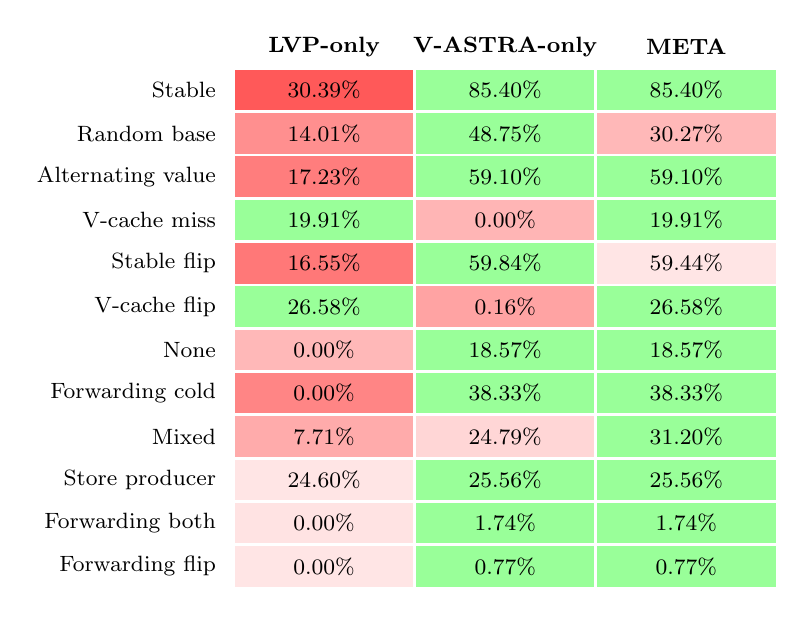
\begin{tikzpicture}[cell/.style={draw=white, line width=1pt,
        minimum width=2.30cm, minimum height=0.55cm, font=\footnotesize}]
    \node[font=\footnotesize\bfseries] at (4.15,0) {LVP-only};
    \node[font=\footnotesize\bfseries] at (6.45,0) {V-ASTRA-only};
    \node[font=\footnotesize\bfseries] at (8.75,0) {META};
    \node[anchor=east, font=\footnotesize] at (2.9,-0.55) {Stable};
    \node[cell, fill=red!65] at (4.15,-0.55) {30.39\%};
    \node[cell, fill=green!40] at (6.45,-0.55) {85.40\%};
    \node[cell, fill=green!40] at (8.75,-0.55) {85.40\%};
    \node[anchor=east, font=\footnotesize] at (2.9,-1.10) {Random base};
    \node[cell, fill=red!44] at (4.15,-1.10) {14.01\%};
    \node[cell, fill=green!40] at (6.45,-1.10) {48.75\%};
    \node[cell, fill=red!28] at (8.75,-1.10) {30.27\%};
    \node[anchor=east, font=\footnotesize] at (2.9,-1.65) {Alternating value};
    \node[cell, fill=red!51] at (4.15,-1.65) {17.23\%};
    \node[cell, fill=green!40] at (6.45,-1.65) {59.10\%};
    \node[cell, fill=green!40] at (8.75,-1.65) {59.10\%};
    \node[anchor=east, font=\footnotesize] at (2.9,-2.20) {V-cache miss};
    \node[cell, fill=green!40] at (4.15,-2.20) {19.91\%};
    \node[cell, fill=red!29] at (6.45,-2.20) {0.00\%};
    \node[cell, fill=green!40] at (8.75,-2.20) {19.91\%};
    \node[anchor=east, font=\footnotesize] at (2.9,-2.75) {Stable flip};
    \node[cell, fill=red!53] at (4.15,-2.75) {16.55\%};
    \node[cell, fill=green!40] at (6.45,-2.75) {59.84\%};
    \node[cell, fill=red!10] at (8.75,-2.75) {59.44\%};
    \node[anchor=east, font=\footnotesize] at (2.9,-3.30) {V-cache flip};
    \node[cell, fill=green!40] at (4.15,-3.30) {26.58\%};
    \node[cell, fill=red!36] at (6.45,-3.30) {0.16\%};
    \node[cell, fill=green!40] at (8.75,-3.30) {26.58\%};
    \node[anchor=east, font=\footnotesize] at (2.9,-3.85) {None};
    \node[cell, fill=red!28] at (4.15,-3.85) {0.00\%};
    \node[cell, fill=green!40] at (6.45,-3.85) {18.57\%};
    \node[cell, fill=green!40] at (8.75,-3.85) {18.57\%};
    \node[anchor=east, font=\footnotesize] at (2.9,-4.40) {Forwarding cold};
    \node[cell, fill=red!48] at (4.15,-4.40) {0.00\%};
    \node[cell, fill=green!40] at (6.45,-4.40) {38.33\%};
    \node[cell, fill=green!40] at (8.75,-4.40) {38.33\%};
    \node[anchor=east, font=\footnotesize] at (2.9,-4.95) {Mixed};
    \node[cell, fill=red!33] at (4.15,-4.95) {7.71\%};
    \node[cell, fill=red!16] at (6.45,-4.95) {24.79\%};
    \node[cell, fill=green!40] at (8.75,-4.95) {31.20\%};
    \node[anchor=east, font=\footnotesize] at (2.9,-5.50) {Store producer};
    \node[cell, fill=red!10] at (4.15,-5.50) {24.60\%};
    \node[cell, fill=green!40] at (6.45,-5.50) {25.56\%};
    \node[cell, fill=green!40] at (8.75,-5.50) {25.56\%};
    \node[anchor=east, font=\footnotesize] at (2.9,-6.05) {Forwarding both};
    \node[cell, fill=red!11] at (4.15,-6.05) {0.00\%};
    \node[cell, fill=green!40] at (6.45,-6.05) {1.74\%};
    \node[cell, fill=green!40] at (8.75,-6.05) {1.74\%};
    \node[anchor=east, font=\footnotesize] at (2.9,-6.60) {Forwarding flip};
    \node[cell, fill=red!10] at (4.15,-6.60) {0.00\%};
    \node[cell, fill=green!40] at (6.45,-6.60) {0.77\%};
    \node[cell, fill=green!40] at (8.75,-6.60) {0.77\%};
    \end{tikzpicture}
    \caption{Cycle reduction relative to NP for LVP-only, V-ASTRA-only,
    and META (\texttt{metaAstraLvpLoads=off}). Green marks the largest
    reduction for each workload. Red shading grows with the gap, in
    percentage points, to that largest reduction.}
    \label{tab:meta-cycle-comparison}
\end{figure}

META matches the better standalone predictor on nine of the twelve
workloads and improves on both for mixed, reducing cycles by
31.20\% relative to NP. However, it underperforms V-ASTRA-only on
random base (24,828 versus 18,249 cycles) and
stable flip (13,039 versus 12,912 cycles). Thus, combining
predictors does not guarantee the best result on every workload.
The performance results alone do not establish the cause of each
difference. The random-base case is examined separately below.

\subsection{Provisional-Base Modes on the Random-Base Workload}
\label{subsec:provisional-base-performance}

The \texttt{metaAstraLvpLoads} parameter was evaluated in
\texttt{off}, \texttt{train}, and \texttt{candidate} modes on the
random-base workload. Figure~\ref{tab:randbase-mode-cycles} shows
the resulting cycle reductions and L1D read misses.

\begin{figure}[H]
    \centering
    \pgfplotsset{rbmode/.style={perfbar, width=0.52\linewidth, height=5.4cm,
        bar width=13pt, enlarge x limits=0.13,
        symbolic x coords={NP,V-ASTRA,off,train,candidate},
        xticklabels={No pred.,V-ASTRA,META off,META train,META cand.},
        xticklabel style={rotate=35, anchor=north east, font=\footnotesize}}}
    \begin{tikzpicture}
    \begin{axis}[rbmode, ymax=60, ylabel={Cycle reduction vs NP (\%)},
        nodes near coords={\pgfmathprintnumber[fixed,precision=2]{\pgfplotspointmeta}}]
        \addplot[fill=metac, draw=metac!70!black] coordinates
            {(NP,0) (V-ASTRA,48.75) (off,30.27) (train,30.57) (candidate,50.80)};
    \end{axis}
    \end{tikzpicture}\hfill
    \begin{tikzpicture}
    \begin{axis}[rbmode, ymax=950, ylabel={L1D read misses}]
        \addplot[fill=candc, draw=candc!70!black] coordinates
            {(NP,800) (V-ASTRA,205) (off,591) (train,587) (candidate,182)};
    \end{axis}
    \end{tikzpicture}
    \caption{Random-base cycle reduction relative to NP (left) and L1D
    read misses (right) across provisional-base modes.}
    \label{tab:randbase-mode-cycles}
\end{figure}

Figure~\ref{tab:randbase-mode-events} shows the corresponding event
counts. The candidate count is reported by
\texttt{vastra.candidates}. In this experiment, it equals the number
of synthetic responses.

\begin{figure}[H]
    \centering
    \begin{tikzpicture}
    \begin{axis}[perfbar, width=0.95\linewidth, height=5.4cm,
        bar width=9pt, ymax=760, enlarge x limits=0.15,
        every node near coord/.append style={font=\tiny, rotate=90, anchor=west},
        ylabel={Count},
        symbolic x coords={V-ASTRA-only,META off,META train,META candidate}]
        \addplot[fill=vac, draw=vac!70!black] coordinates
            {(V-ASTRA-only,595) (META off,209) (META train,213) (META candidate,618)};
        \addplot[fill=lvpc, draw=lvpc!70!black] coordinates
            {(V-ASTRA-only,0) (META off,386) (META train,386) (META candidate,182)};
        \addplot[fill=candc, draw=candc!70!black] coordinates
            {(V-ASTRA-only,0) (META off,0) (META train,386) (META candidate,182)};
        \addplot[fill=npc, draw=npc!70!black] coordinates
            {(V-ASTRA-only,0) (META off,386) (META train,0) (META candidate,0)};
        \legend{V-ASTRA candidates, LVP committed loads,
                Provisional bases, Base unavailable}
    \end{axis}
    \end{tikzpicture}
    \caption{Random-base event counts. Every provisional base was
    validated and none was dropped. V-ASTRA-only has no LVP.}
    \label{tab:randbase-mode-events}
\end{figure}

Train mode changes the cycle count by only 106 cycles relative to
off (24,722 versus 24,828). Candidate mode reduces cycles by 7,310
(29.4\%) relative to off and by 731 relative to V-ASTRA-only. It
also reduces L1D read misses from 591 to 182 and increases synthetic
responses from 209 to 618. The number of committed LVP-speculated
loads falls from 386 in off and train to 182 in candidate mode.

These counters are consistent with candidate mode restoring
V-ASTRA opportunities for some LVP-served loads. However, they do
not establish how much of the cycle reduction is caused by individual
additional bypasses. Candidate counts alone are also not a reliable
indicator of performance: on mixed, candidates increase from
390 to 988 while synthetic responses remain at 191 and cycles do not
change. On V-cache miss, candidates increase from 200 to 800, but
no synthetic responses occur and cycles remain unchanged.

The random-base experiment was repeated after the alignment retry
fix, with one run per mode. The off, train, and candidate cycle counts
exactly reproduced the five-run results.

\subsection{Performance of Dependency-Handling Designs}
\label{subsec:dependency-performance}

The performance harness uses the default memory-FU timing
(\texttt{extraAssumedLat = 2}), under which Design~A's scoreboard
release is inactive.

Design~B forwarding is enabled in the V-ASTRA performance mode, but
no V-ASTRA-without-forwarding control is available. Its contribution
therefore cannot be isolated. Figure~\ref{tab:forwarding-performance}
reports the combined configuration relative to NP. Forwarded
consumer counts are from \texttt{vastra.fwdAdmitted} and represent
admitted consumers, not committed instructions.

\begin{figure}[H]
    \centering
    \begin{tikzpicture}
    \begin{axis}[perfbar, width=0.85\linewidth, height=5.2cm,
        bar width=22pt, ymax=45, enlarge x limits=0.18,
        ylabel={Cycle reduction vs NP (\%)},
        symbolic x coords={fc,mx,fb,ff},
        xticklabels={{Forwarding cold\\(188 fwd.)},{Mixed\\(188 fwd.)},
                     {Forwarding both\\(400 fwd.)},{Forwarding flip\\(394 fwd.)}},
        xticklabel style={align=center},
        nodes near coords={\pgfmathprintnumber[fixed,precision=2]{\pgfplotspointmeta}\%}]
        \addplot[fill=vac, draw=vac!70!black] coordinates
            {(fc,38.33) (mx,24.79) (fb,1.74) (ff,0.77)};
    \end{axis}
    \end{tikzpicture}
    \caption{Cycle reduction of V-ASTRA (with forwarding) relative to NP
    on the forwarding workloads. The number of forwarded consumers
    (\texttt{vastra.fwdAdmitted}) is given under each workload.}
    \label{tab:forwarding-performance}
\end{figure}

Forwarding cold reduces cycles by 38.33\% while L1D misses remain
unchanged at 400, despite 191 synthetic responses. This is consistent
with a benefit from overlap, although the measurements do not isolate
its contribution. The gains on forwarding both and forwarding flip
are smaller (1.74\% and 0.77\%), with path-padding spreads of
approximately 0.059\% and 0.152\%, respectively.

\subsection{Threats to Validity and Interpretation}
\label{subsec:performance-limitations}

The results are deterministic microbenchmark measurements on a single
MinorCPU, cache, and memory configuration. They do not represent
application-level speedups. The repeated runs check sensitivity to
output-path layout only and are not independent statistical samples.
Design~A was not measured under the default timing, and the
contribution of Design~B cannot be separated from V-ASTRA. Small
effects close to the observed layout variation should therefore be
interpreted with caution.

Overall, the cycle reductions are substantial but depend on the
workload. META improves on both standalone predictors on mixed, but is
slower than V-ASTRA-only on random base and stable flip. Candidate mode
gives a large improvement on random base, but its broader benefit is not
established by these workloads.

\section{Limitations and Differences from the Original Paper}

This implementation adapts the paper's prediction mechanisms to
gem5 MinorCPU rather than reproducing its complete architecture
and evaluation environment~\cite{ravenel2025architecting}. The
differences in processor organization, prediction timing, and
evaluation methodology affect the resulting behavior and
performance.

\subsection{Processor Model and Evaluation Scope}

The implementation uses gem5 MinorCPU and targeted RISC-V
microbenchmarks, whereas the paper uses a modified CVA6-based
processor and SPEC CPU2017 SimPoint evaluation. The paper's
processor is four-wide, with a 32-entry scoreboard, and can issue two
loads per cycle~\cite{ravenel2025architecting}. The MinorCPU
configuration used here is also four-wide but issues at most one memory
instruction per cycle, and its scoreboard tracks every architectural
register rather than a fixed number of entries.

Consequently, the evaluations differ in processor organization,
pipeline constraints, cache configurations, and workloads. The
reported cycle reductions characterize the tested simulator
configurations and deterministic microbenchmarks, not general
application-level speedups, and should not be compared directly
with the paper's performance results.

The value-cache features also support only a single CPU, a single
hardware thread, and syscall-emulation mode, and virtual synonyms,
uncacheable accesses, and compressed loads were not evaluated.

\subsection{Differences from the Original Design}

The LVP predictor table and its confidence policy follow the paper: a
direct-mapped, untagged, PC-indexed table with a two-bit saturating
counter~\cite{ravenel2025architecting}.

The differences lie primarily in prediction use and recovery. The
implementation consumes an LVP prediction only as the base operand of
an eligible dependent integer load. The consumer must be the oldest
unsent memory operation, while its producer must be the oldest
in-flight instruction, carry a prediction, have already entered the
LSQ, and still be awaiting its response. The prediction is validated against the producer's
actual value when its response arrives. If an incorrect prediction was
used, the implementation redirects execution and refetches younger
instructions rather than reproducing the paper's scoreboard-based
replay mechanism.

The ASTRA predictor retains full 64-bit base addresses. The paper's
Last Address Compressed Table (LACT) is a 32-entry LRU address
compressor: a compact 5-bit identifier represents the upper 44 bits,
while the lower 20 bits are retained in the predictor entry. The
paper reports an 85\% reduction in predictor storage from this
representation~\cite{ravenel2025architecting}. The implementation
does not include this compression mechanism. Similarly, the paper's value-cache tags reuse the region
identifier with 8 additional bits, whereas the implementation uses
full virtual-page-number tags. The paper reports a 75\% tag-storage
reduction from its compressed representation
~\cite{ravenel2025architecting}. Although the implemented value cache has the same 4-KiB capacity and 16-byte entry
geometry, it uses per-byte validity information, does not implement a
16-byte line-fill mechanism, and invalidates or falls back for certain
special and cross-line accesses.

V-ASTRA candidacy is decided in Execute when the load initiates its
memory access. At this point, the predicted base is compared with the
actual base and older in-flight stores are scanned for potential
conflicts. This candidate decision does not immediately authorize a
bypass. The final bypass is accepted in the LSQ only after
address translation and the store-buffer check. The implementation
then checks the effective address, repeats the older-store scan using
the actual access size, verifies the saved value-cache snapshot, and
performs a fresh value-cache lookup. If any check fails, the load falls
back to the normal memory path. In contrast, the paper performs
address validation at issue, allowing eligible dependents to issue in
the same cycle as the load.

For store safety, the implementation uses explicit scans of older
in-flight stores and atomics, together with the existing store-buffer
checks. The scan is performed both when forming a V-ASTRA candidate
and when the request is considered for bypass. This differs from the
paper's counting Bloom filter (CBF) and in-flight invalidation FIFO,
which track potential conflicts with outstanding stores
~\cite{ravenel2025architecting}. The exact
scan avoids the CBF's set-granularity false positives, although its
cost grows with the number of in-flight stores. The FIFO is not
required by the current MinorCPU path because older memory references
are issued in order and their store addresses are known by the
candidate decision point.

The implementation also omits the paper's L0 minicache. The paper
describes a 32-entry direct-mapped VIPT load/store-allocate structure
with separate speculative and committed data arrays, per-byte
validity, and line locking from execution through commit. It provides
a fast path for loads affected by in-flight stores and supports
speculative store-to-load forwarding~\cite{ravenel2025architecting}. In the
current implementation, loads rejected because of older-store conflicts fall back to the
normal memory path. MinorCPU's existing store buffer can forward fully
covered loads, while partial coverage must wait. The minicache would
therefore add functionality beyond the current value cache and bypass
path.

The dependency mechanisms also differ from the paper's early-execution
model. Design~A releases the scoreboard dependency associated with a
bypassed load, allowing a dependent instruction to become eligible
earlier under the stall-on-use timing configuration. It does not
forward a predicted value: the dependent still reads the committed
register value. Under the default timing configuration, this release
mechanism is inactive. Design~B forwards a validated V-ASTRA value as
the base operand of an eligible dependent integer load. It does not
provide general forwarding to arbitrary ALU, branch, store, or
floating-point instructions. Non-memory dependent instructions
continue to execute at in-order commit, after their producer commits.

Both designs recover
only when a wrong prediction was actually used. A wrong prediction that
was never consumed requires no recovery in either. The difference lies
in the recovery mechanism: the paper replays younger instructions
through its scoreboard, whereas this implementation squashes younger
instructions and redirects execution to refetch them.

\subsection{Future Work}

Future work covers project-specific extensions, components from the
original design, and broader evaluation.

\paragraph{Further development of project-specific extensions.}
The random-base result motivates an adaptive admission policy for
provisional LVP-derived bases, potentially using LVP confidence,
recent validation outcomes, or agreement with ASTRA predictions.
It should be evaluated on random base, stable flip, V-cache flip, mixed,
and forced-misprediction workloads to assess gains and regressions.
Further evaluation should isolate Design~B by comparing V-ASTRA
with forwarding enabled and disabled, and measure Design~A under
stall-on-use timing. Design~B could also be extended to additional
load operand positions and store addresses. Forwarding to ALU and
branch instructions would require more substantial changes to
MinorCPU's execution model.

\paragraph{Architectural extensions toward the original design.}

The most substantial omitted component is the speculative L0
minicache. It could provide a fast path for store-dependent loads
currently rejected by V-ASTRA, using speculative and committed data
arrays with store-to-load forwarding. Its implementation would
require LSQ integration, speculative-store handling, line locking,
and recovery on stream changes. Its benefit should be evaluated
using store-heavy workloads and in combination with META.

Another extension is LACT-based address compression. The paper's
32-entry LRU compressor maps 5-bit region identifiers to upper
address bits while retaining 20 low bits in LAT entries. The
value-cache tag reuses the identifier with 8 additional bits. The
paper reports 85\% lower predictor storage and 75\% lower tag
storage. The current implementation instead stores full 64-bit
bases and full virtual-page tags. Implementing LACT would require
identifier allocation and recycling, compressed LAT and value-cache
tags, cache invalidation on identifier recycling, and rejection of
predictions whose displacement carries out of the compressed
region. This is primarily a storage-efficiency and architectural
fidelity extension.

Other possible changes include replacing the exact older-store scan
with the paper's counting Bloom filter (CBF) and invalidation FIFO,
and replacing squash-and-refetch recovery with scoreboard replay.
These are lower priority: the current scan is exact, while replay
would require substantial changes to MinorCPU's reissue and
scoreboard-restoration mechanisms. Further directions discussed
in the paper include VTAGE, process-ID-tagged value-cache entries,
multiprocessor support, and security analysis
\cite{ravenel2025architecting}.

\paragraph{Broader performance evaluation.}

The current evaluation uses deterministic microbenchmarks and a
single main processor and memory configuration. Future work should
include application-level and embedded benchmarks, broader cache
and memory-latency configurations, and different processor timing
parameters and widths where supported. Supporting compressed
RISC-V loads would also improve coverage of binaries built for
\texttt{rv64gc}. Multicore and full-system support would require
additional coherence and external-writer mechanisms, making them
larger extensions beyond the current scope.

\section{Conclusion}

This project implemented and evaluated value-prediction mechanisms
in gem5 MinorCPU, including Last Value Prediction (LVP),
ASTRA-based load-base prediction, a dedicated value cache, and
guarded V-ASTRA load bypass. It also investigated two
dependency-handling mechanisms: Design~A releases scoreboard
dependencies after a successful bypass, while Design~B forwards
validated values to eligible dependent loads.

The paper's META predictor was adapted to MinorCPU to select
between LVP and V-ASTRA on a per-consumer basis. Validated
V-ASTRA values are preferred, while consumers wait when a
V-ASTRA result is Pending rather than immediately falling back
to LVP. LVP may be selected when the V-ASTRA outcome has failed
or is absent and the LVP admission conditions are satisfied. The implementation also introduces experimental
provisional-base modes that use LVP-derived information for
ASTRA training and V-ASTRA candidate generation.

Performance measurements on deterministic microbenchmarks show
that prediction effectiveness depends on workload characteristics.
META achieves a 31.20\% cycle reduction on mixed,
outperforming both standalone predictors. However, on
random base, default META achieves 30.27\%, compared with
48.75\% for V-ASTRA-only, and it also performs slightly worse
than V-ASTRA on stable flip. The experimental candidate
mode improves the random-base reduction to 50.80\%, but this
benefit is workload-specific and does not generalize across the
evaluated workloads. These results characterize the tested simulator
configurations, not application-level speedups. Design~A was
validated under stall-on-use but not performance-evaluated in
that configuration, while the contribution of Design~B was not
isolated from V-ASTRA.

Validation covered predictor behavior, value-cache correctness,
memory ordering, dependency handling, and misprediction recovery.
The experiments demonstrated that unused incorrect LVP predictions
do not require recovery and that V-ASTRA-served consumers do not
trigger LVP recovery. They also exposed and helped correct a
provisional-state cleanup defect on early alignment faults.

Overall, this work demonstrates the challenges of integrating
value prediction into an in-order processor, particularly the
interactions between speculative operands, address prediction,
value-cache bypass, memory ordering, dependency tracking, and
recovery. It provides a basis for further investigation of value
prediction in MinorCPU. Important next steps include completing
final-source validation, implementing architectural components
such as the speculative L0 minicache and LACT, improving provisional
candidate admission, and evaluating the mechanisms on more
representative workloads.


\bibliographystyle{plain}
\bibliography{references}

\end{document}
